\section{Introduction}

Major hurricanes are becoming more intense under the effect of global warming \citep{bhatia2019recent, knutson2020tropical}. Better understanding their repercussions on coastal areas becomes therefore critical. However, estimating the impact of hurricanes on the coastal ocean circulation remains a challenge. Understanding wave-current interactions and representing their impact on coastal ocean transport processes is central to many coastal activities such as dredging, erosion management, oil and gas activities, search and rescue, and insurance \citep{bever2013simulating,li1998three, breivik2013advances}. All these activities require wave-current models to predict the impact of tropical cyclones on the coastal circulation and on the sea surface elevation.

Wave-current interactions during a cyclone are highly nonlinear and vary significantly in space and time \citep{wu2011fvcom}. Wave-induced currents are generated by wave radiation stress gradients \citep{longuet1970longshore}, affecting water levels near shorelines and wave breaking points \citep{longuet1964radiation}. Changes in water levels and currents, in turn, affect the motion and evolution of the waves \citep{sikiric2013coupling}. Coupled wave-current models hence require the calculation of the full directional wave spectrum in order to correctly reproduce the dynamics of wind-driven surface waves. This is usually achieved by spectral wave models, which describe the evolution of the wave energy spectrum. As of today, the most popular spectral wave models are the WAve Model (WAM) \citep{group1988wam}, %TOMAWAC \citep{benoit1997tomawac},
Simulating WAve Nearshore (SWAN) \citep{booij1999third}, and WAVEWATCH III \citep{tolman2009user}. Among these models, SWAN has been specifically developed for coastal applications, as it represents depth-induced wave breaking and triad wave-wave interactions using numerical techniques adapted to small-scale, shallow water regions \citep{booij1999third}. WAVEWATCH III has also recently been equipped with new parallelization algorithm, domain decomposition and numerical schemes for high resolution coastal applications \citep{ww3dg,abdolali2020large}.

Coastal oceans are characterized by the complex topography of the coastline and the presence of islands, reefs and artificial structures. Traditional structured-grid models lack the flexibility to simulate near-shore processes at a sufficiently small scale. Although the use of nested structured grids allows local grid refinement \citep{warner2010development}, staircase-like representation of complex coastal topographies cannot be avoided. Instead, unstructured-mesh models easily adapt to the topography and are hence better suited to coastal processes \citep{fringer2019future}. Capturing the impact of the topography on wave interactions becomes even more important in the case of tropical cyclones. Heavy winds generate large wind-waves and disturb ocean conditions \citep{liu2020impacts} by causing coastal upwellings on continental shelves \citep{smith1982response} and inducing strong currents, waves and storm surges in nearshore and coastal regions \citep{dietrich2010high, weisberg2006hurricane}. 

Ocean waves act as the dynamical interface between the atmosphere and the ocean. Through this interface, tropical cyclones cause a cooling of the upper ocean layer by vertical mixing and heat transfer \citep{aijaz2017nonbreaking,varlas2020investigating}. By altering the structure of the upper-ocean, hurricane can cause the disruption of major ocean currents such as the Florida Current and Gulf Stream \citep{oey2007hurricane}. Interaction with hurricanes alters the thermal structure of these currents and can cause a significant decline of their flow, resulting in delayed increased coastal levels along their path, even in locations out of reach of the hurricane itself \citep{ezer2017observations, ezer2018interaction,ezer2020long}.

Near the storm, heavy wind conditions also affect material transport at the ocean surface. The transport of drifting objects or substances that are locally released is often best represented by a Lagrangian individual-based model. Such an approach is routinely used to model the dispersal of larvae, pollutants, sediments and many other tracers (e.g. \citealp{le2012surface,liubartseva2018tracking, figueiredo2013synthesizing,frys2020fine}). Although some transport model might take wave-induced currents into account, most of them neglect wave-current interactions, which can lead to significant errors in storm conditions \citep{rohrs2012observation,curcic2016hurricane}. \cite{niu2017role} and \cite{mao2018wave,mao2020particle} investigated the impact of wave-current interactions during storm event in lakes and inlets. However, to our knowledge, there have been no similar studies on the impact of hurricane-induced wave-current interactions in coastal environments such as the Florida Reef Tract (FRT), where changes in transport processes might significantly impact the biological connectivity.

The main questions we want to answer in this study are the following: (1) How important are wave-current interactions during a tropical cyclone? (2) What effect do they have on the transport of drifting material? We tackle these issues by investigating the transport of drifting particles on the Florida shelf during Hurricane Irma, one of the strongest and costliest tropical cyclones on record in the Atlantic Basin \citep{xian2018brief}, which made landfall in Florida in September 2017. To do that, we developed an unstructured-mesh coupled wave-current model of the whole FRT to simulate the ocean circulation under hurricane conditions. Both modeled currents and waves were validated against field measurements and then used to simulate the transport of drifting material in the Florida Keys and over the Florida inner shelf. Model outputs were then compared with uncoupled simulation results in order to assess the impact of the radiation stress gradient and Stokes drift on the modeled currents and transport.  

% === METHODS === %
\section{Methods}
\subsection{Study area and observational data}
We study the ocean circulation in an area that covers the whole FRT and includes the nortwestern end of the Gulf of Mexico and the Straits of Florida (Fig. \ref{fig:mesh}). The large-scale ocean circulation around South Florida is dominated by the Florida Current (FC), which originates from the Loop Current (LC) where it enters the Florida Straits from the Gulf of Mexico, and, downstream, forms the Gulf Stream. The FC is a major western boundary current characterized by spatial variability and meandering, associated with the presence of cyclonic eddies between the core of the current and the complex reef topography of the FRT \citep{lee1995florida,kourafalou2012florida}. The variability of the FC extends over a large range of spatial and temporal scales, with periods of 30-70 days in the Lower Keys \citep{lee1995florida} and shorter periods of 2-21 days in the Upper Keys \citep{lee1977low}, and exhibits significant seasonal and interannual cycles \citep{johns1987meandering, lee1988wind,schott1988variability}. Circulation on the West Florida Shelf (WFS), on the other hand, is forced by local winds and tidal fluctuations \citep{lee2002volume,liu2012seasonal}. Furthermore, due to its location relative to the warm waters of the North Atlantic, Florida is particularly vulnerable to tropical cyclones. On average, the state is hit by a hurricane every two years and strong hurricanes, some of which are among the most destructive on record, strike Florida on average once every four years \citep{malmstadt2009florida}.

The state of the ocean around Florida is monitored by an extensive array of tide gauges, current meters and buoys. In this study, we used sea surface elevation measurements from the National Oceanic and Atmospheric Administration’s (NOAA) Tides and Currents dataset. These measurements were taken at four locations: two in the Florida Keys (Key West and Vaca Key); one on the East coast of Florida (Virginia Key); and one on the West coast (Naples). For the currents, we used ADCP measurements from the University of South Florida's College of Marine Science's (USF/CMS) Coastal Ocean Monitoring and Prediction System (COMPS) for the WFS \citep{weisberg2009mean}. More specifically, we used measurements from moorings C10, C12 and C13, respectively located at the 25, 50, and 50 m isobaths of the WFS \citep{liu2020impacts}. Finally, for the waves, we used measurements from four buoys of the NOAA's National Data Buoy Center (NDBC); two on Florida's eastern shelf and two on the WFS. The locations of all measurement stations are shown in Fig. \ref{fig:mesh}.

\begin{figure}
    \centering
    \includegraphics[width=\textwidth]{chapters/irma/figures/fig_mesh_hurr.png}
    \caption{(\textbf{A}) Mesh of the computational domain with the trajectory of Irma. The category of the hurricane is given by the Saffir-Simpson color scale. (\textbf{B}) Bathymetry of the domain with the location of stations used for the validation of the model outputs. (\textbf{C}) Close up view of the Lower Keys area (red box in (A)), where the mesh resolution reaches 100 m near reefs (shown in dark orange) and islands (shown in dark grey)}
    \label{fig:mesh}
\end{figure}

\subsection{Wind and atmospheric pressure during Hurricane Irma}

Hurricane Irma made landfall in Florida on 10 September 2017 as a category 4 hurricane at Cudjoe Key (Florida Keys) and later as a category 3 hurricane on Marco Island, south of Naples (see hurricane track in Fig. \ref{fig:mesh}). It then weakened to a category 2 hurricane as it moved further inland \citep{irmaNOAA}. The storm damaged up to 75\% of the buildings at its landfall point in the Florida Keys, making it one of the strongest and costliest hurricanes on record in the Atlantic basin \citep{xian2018brief,zhang2019modeling}. The strongest reported sustained winds on Marco Island were 50 m/s while the highest recorded storm surge was 2.3 m, although larger wind speed likely occurred in the Florida Keys \citep{pinelli2018overview}. To reproduce the wind profile of Irma in our model, we used high-resolution H$^\ast$Wind wind fields \citep{powell1998hrd}. As these data represent 1-min averaged wind speeds, we multiplied them by a factor 0.93 to obtain 10-min averaged wind speeds \citep{harper2010guidelines}. This operation reduces the erratic values caused by the greater variance of mean winds measured over periods shorter than 10 minutes. Furthermore, H*Wind wind profiles did not cover the whole model extent during the passage of the hurricane and were thus blended within a coarser wind field extracted from the European Centre for Medium-Range Weather Forecasts (ECMWF) ERA-5 dataset (Fig. \ref{fig:atm}A). The pressure field during the passage of Hurricane Irma was also reconstructed using ERA-5 data. However, the coarse resolution of the dataset smoothes out the depression at the center of the hurricane, leading to an underestimation of the pressure gradient (Fig. \ref{fig:atm}B). To better capture the central depression of Irma, we therefore built a hybrid pressure field using the position and the minimal pressure of the core of the hurricane based on its track, as recorded in the HURricane DATabases (HURDAT) 2 \citep{landsea2013atlantic}. Based on this information, the hybrid pressure field was constructed by combining an idealized Holland pressure profile \citep{lin2012hurricane} within the radius of maximum wind speed of Irma \citep{knaff2018statistical} with ERA-5 pressure field. The transition from the Holland profile to ERA-5 data outside the radius of maximum wind speed data was performed using a smooth step function (Fig. \ref{fig:atm}).

\begin{figure}
    \centering
    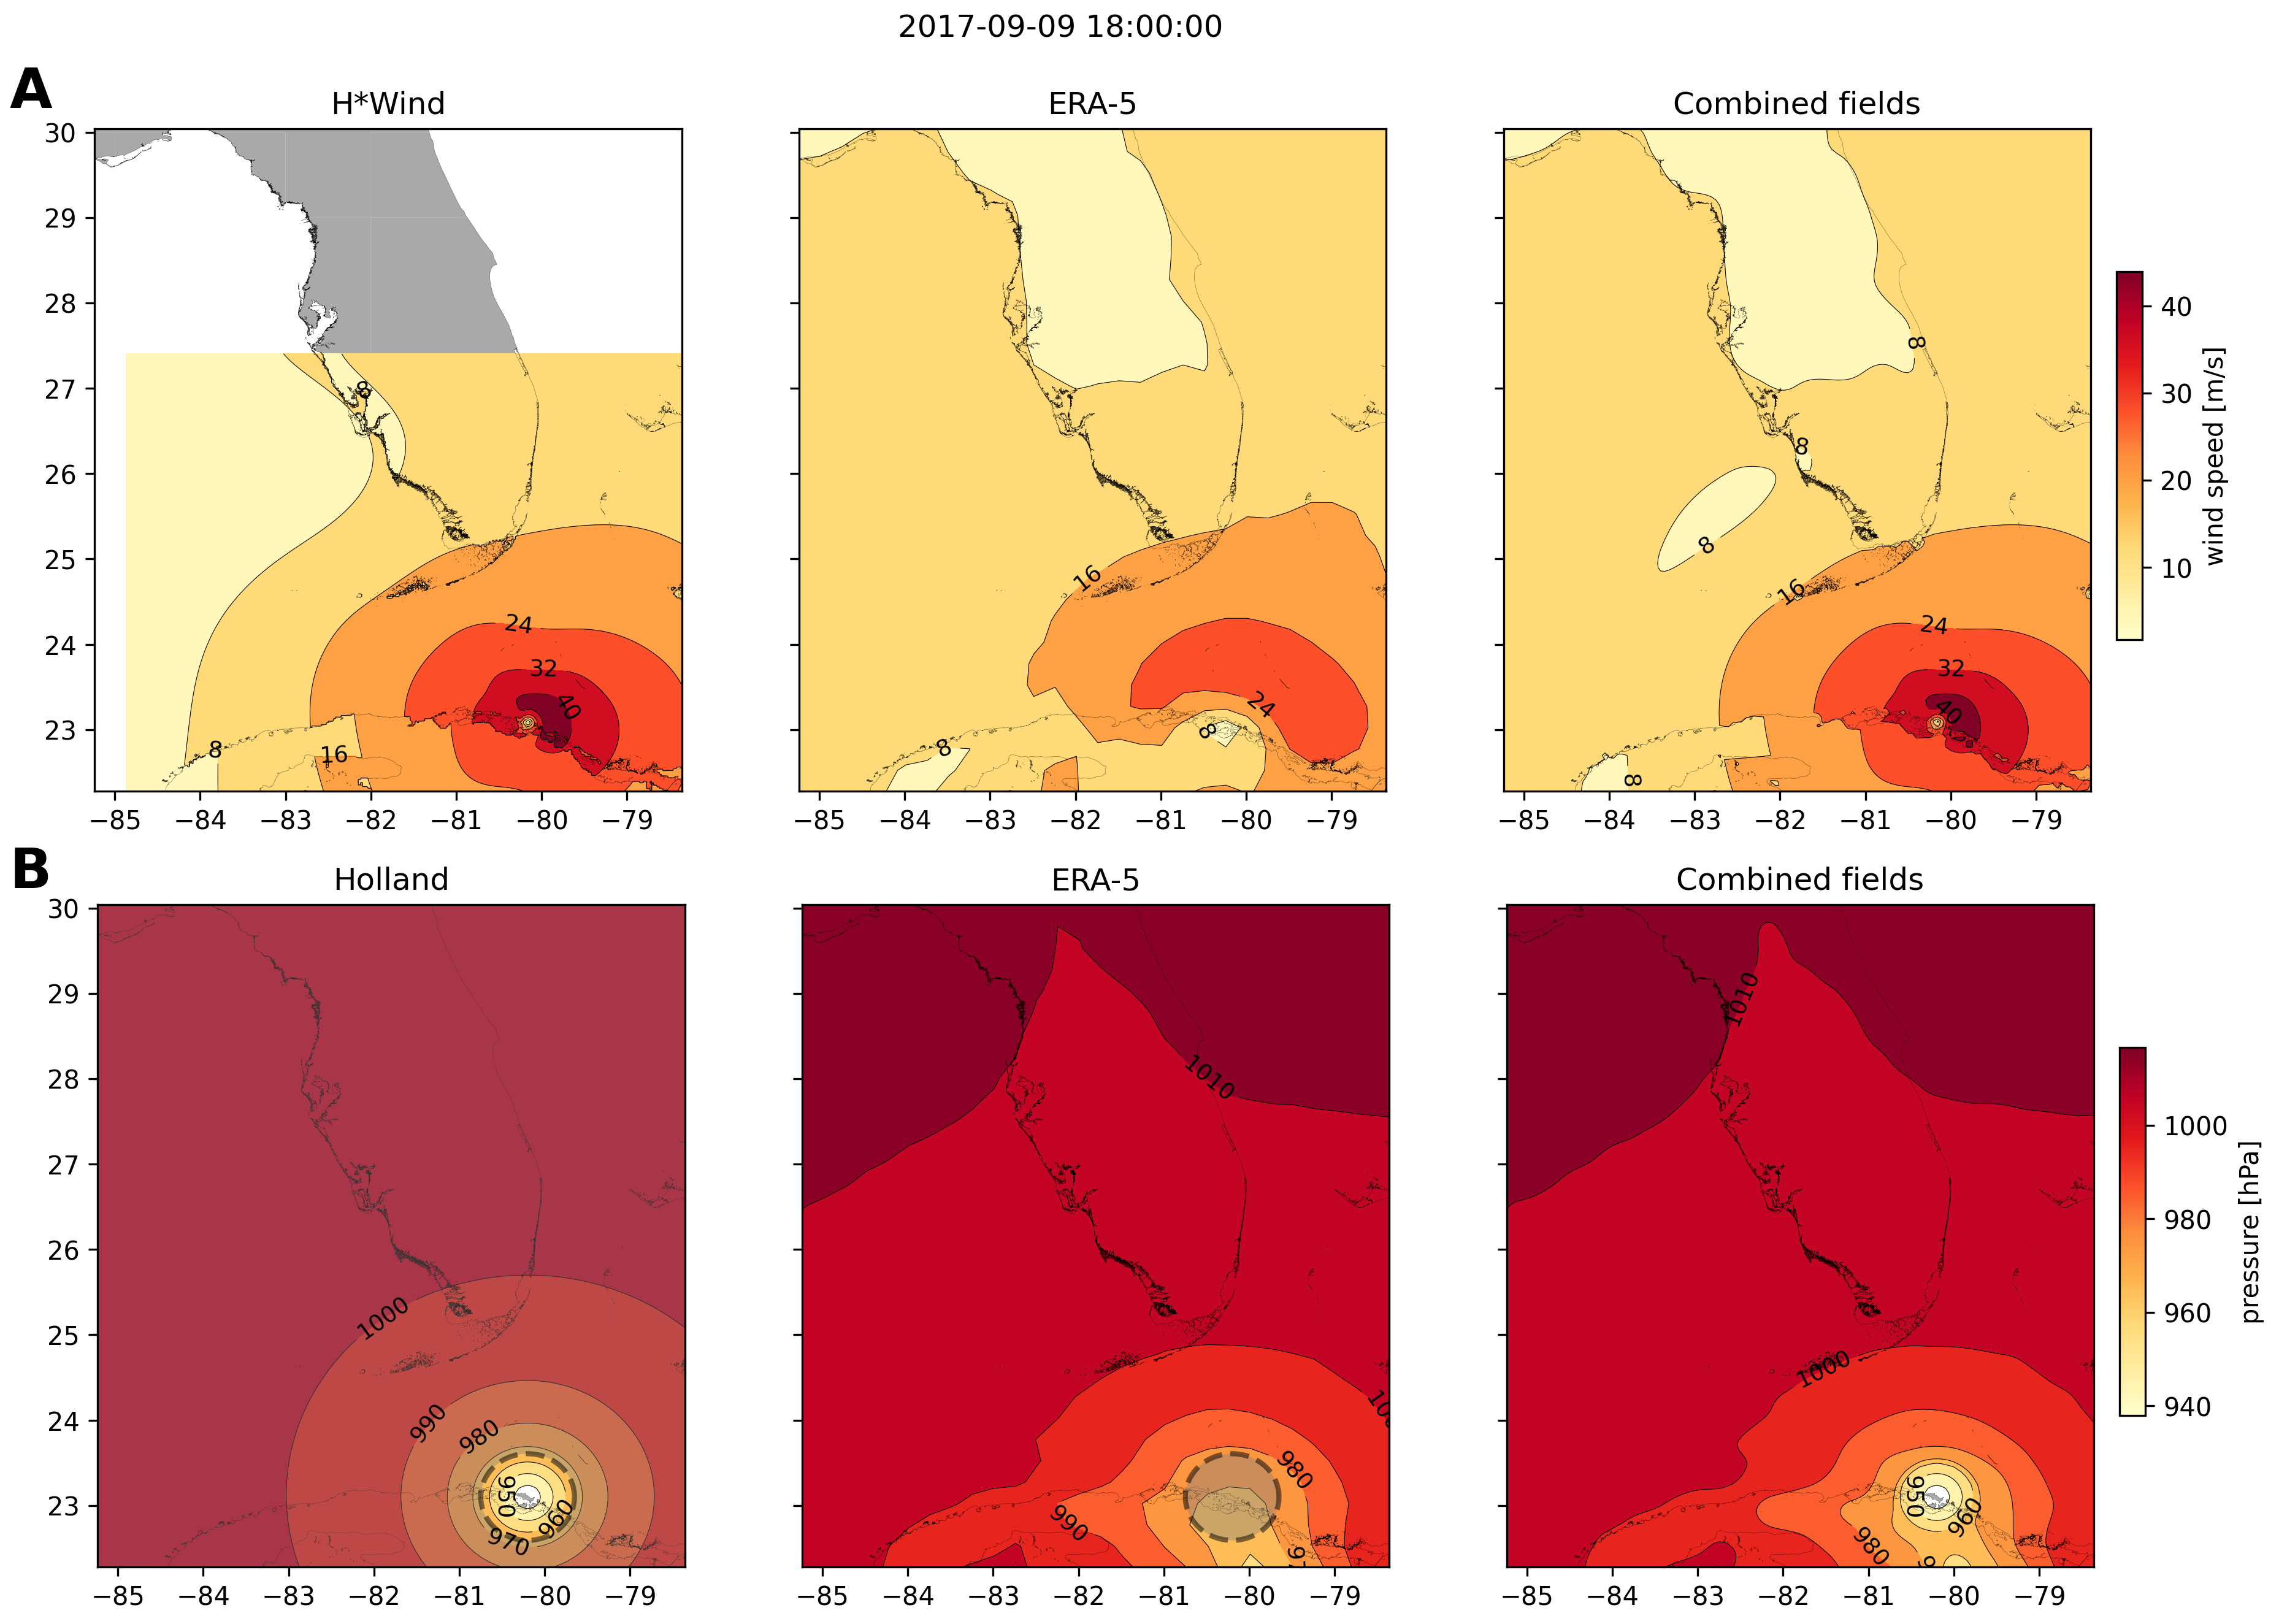
\includegraphics[width=.99\textwidth]{chapters/irma/figures/hwind+holland_vs_era.png}
    \caption{Snapshot of the hybrid wind (\textbf{A}) and pressure (\textbf{B}) profiles constructed to capture the passage of Hurricane Irma at 1800 UTC on 9 September 2017. Wind profiles were obtained by combining high resolution H*Wind with coarser ERA-5 wind fields. The pressure field was built by combining the ERA-5 pressure field with an idealized Holland pressure profile based on the track of Irma in the HURDAT 2 database. Holland field was only used within the radius of maximum wind speed (dashed grey line) of the hurricane to capture its central depression. }
    \label{fig:atm}
\end{figure}

\subsection{Hydrodynamic model}

Ocean currents generated during Hurricane Irma around South Florida were modeled using the 2D barotropic version of the unstructured-mesh Second-generation Louvain-la-neuve Ice-ocean Model\footnote{\url{https://www.slim-ocean.be}} (SLIM) \citep{lambrechts2008multi}. The model mesh covers an area similar to the model extent of \cite{dobbelaere2020coupled}, that includes the FRT but also the Florida Straits and part of the Gulf of Mexico (Figure \ref{fig:mesh}). However, this area has been slightly extended northeastward and westward in order to include the NOAA-NDBC buoys. Furthermore, to withstand potential cell drying during the hurricane, we solved the conservative shallow water equations with wetting-drying:
\begin{equation}
    \begin{split}
        \dfrac{\partial H}{\partial t} +\nabla\cdot(\UV) =& ~0~, \\
        \dfrac{\partial \UV}{\partial t}  + \nabla\cdot\left(\dfrac{\UV\UV}{H}\right) + f\mathbf{e}_z \times \UV =& ~\alpha gH\nabla(H-h) - \dfrac{1}{\rho}\nabla p_\text{atm} + \dfrac{1}{\rho}\text{\boldmath$\tau$}_s \\
         &+\nabla\cdot(\nu\nabla\UV) - \dfrac{C_b}{H^2}|\UV|\UV + \gamma(\UV_\text{ref}-\UV)~,
    \end{split} \label{eq:slim}
\end{equation}
where $H$ is the water column height and $\UV$ is the depth-averaged transport; $f$ is the Coriolis coefficient; $g$ is the gravitational acceleration; $h$ is the bathymetry; $\alpha$ is a coefficient indicating whether the mesh element is wet ($\alpha=1$) or dry ($\alpha=0$) \citep{le2020implicit}; $\nu$  is the Smagorinsky viscosity; $C_b$ is the bulk bottom drag coefficient; $p_\text{atm}$ is the atmospheric pressure; {\boldmath$\tau$}$_s$ is the surface stress, usually due to wind; and $\gamma$ is a relaxation coefficient towards a reference transport $\UV_\text{ref}$. As this study focuses on transport processes and not coastal flooding, wetting-drying is only applied on wet grid cells that may become dry under the influence of the hurricane. As in \cite{frys2020fine} and \cite{dobbelaere2020coupled}, SLIM currents were gradually relaxed towards the operational Navy HYbrid Coordinate Ocean Model (HYCOM) product (GOMl0.04\footnote{\url{https://www.hycom.org/data/goml0pt04}}, \cite{chassignet2007hycom}) in regions where the water depth exceeds 50 m. HYCOM's 3D currents were depth-integrated into 2D transports to be used as forcing in the model. Moreover, these transports as well as HYCOM's sea surface elevation were used as boundary condition in the model.

We adapted the parameterization of the wind-induced surface stress to storm conditions. At very high wind speeds, the white cap is blown off the crest of the waves. This phenomenon, also known as spume, has been hypothesized to generate a layer of droplets that acts as a slip layer for the winds at the ocean-atmosphere interface \citep{holthuijsen2012wind}. It causes a saturation of the wind drag coefficient for strong winds \citep{powell2003reduced,donelan2004limiting,curcic2020revised}. We take this saturation effect into account by using the wind  drag parameterization of \cite{moon2007physics}. In this parameterization, the drag coefficient $C_d$ depends on the wind speed at 10-m height $U_{10}$ according to:
\begin{equation}
    C_d = \kappa^2 \log\left(\dfrac{10}{z_0}\right)^{-2}\label{eq:drag}
\end{equation}
where $\kappa$ is the von Karman constant and $z_0$ is the roughness length expressed as: 
\begin{equation}
    z_0 =\left\{\begin{array}[]{ll}
        \dfrac{0.0185}{g}u_{\ast}^2 & \text{if }U_{10} \leq 12.5\text{ m/s}~, \\
        \lbrack 0.085(-0.56u_{\ast}^2+20.255u_{\ast} & \text{if }U_{10} > 12.5\text{ m/s}~, \\
        \quad +2.458) - 0.58\rbrack\times 10^{-3} 
    \end{array}\right.
\end{equation}
with $u_\ast$ the friction velocity. The relation between $U_{10}$ and $u_{\ast}$ is given by:
\begin{equation}
    U_{10}=-0.56u_{\ast}^2+20.255u_{\ast}+2.458~.
\end{equation}

The mesh resolution depends on the distance to the coastlines and reefs following the approach of \cite{dobbelaere2020coupled}. The mesh is then further refined according to bathymetry value and gradient, as suggested in the SWAN user-guide\footnote{\url{http://swanmodel.sourceforge.net/unswan/unswan.htm}}. Such an approach improves the model efficiency as the mesh resolution is only increased where required by the currents and waves dynamics. The mesh was generated with the seamsh\footnote{\url{https://pypi.org/project/seamsh/}} Python library, which is based on the the open-source mesh generator GMSH \citep{geuzaine2009gmsh}. It is composed of approximately 7.7 $\times$ 10$^5$ elements. The coarsest elements, far away from the FRT, have a characteristic length of about 5 km whereas the finest elements have a characteristic length of about 100 m along the coastlines and over the reefs (Fig \ref{fig:mesh}).

\subsection{Wave model}
Waves were modeled using the parallel unstructured-mesh version of the Simulating WAves Nearshore (SWAN) model \citep{booij1999third}, one of the most popular wave models for coastal areas and inland waters. It solves the action balance equation \citep{mei1989applied}:
\begin{equation}
    \dfrac{\partial N}{\partial t} + \nabla_\mathbf{x}\cdot[(\mathbf{c}_g+\mathbf{u})N] + \dfrac{\partial }{\partial \theta}[c_\theta N] + \dfrac{\partial}{\partial \sigma}[c_\sigma N] = \dfrac{S_{in}+S_{ds}+S_{nl}}{\sigma}~, \label{eq:swan}
\end{equation}
where $N=E/\sigma$ is the wave action density and $E$ is the wave energy spectrum; $\theta$ is the wave propagation direction; $\sigma$ is the intrinsic wave frequency; $\mathbf{c}_g$ is the wave group velocity, $\mathbf{u}=\mathbf{U}/H$ is SLIM depth-averaged current velocity; $c_\theta$ and $c_\sigma$ are the propagation velocities in spectral space due to refraction and shifting in frequency due to variations in depth and currents; and $S_{in}$, $S_{ds}$, and $S_{nl}$ respectively represent wave growth by wind, wave decay and nonlinear transfers of wave energy through four and three-wave interactions, \ie~quadruplets and triplets. The wave spectra were discretized with 48 direction bins and 50 frequency bins logarithmically distributed from 0.03 to 2 Hz. Exponential wind growth was parameterized using the formulation of \cite{janssen1991quasi}, while dissipations by whitecapping and bottom dissipation followed the formulations of \cite{komen1984existence} and \cite{madsen1989spectral}, respectively.

Coefficients for exponential wind growth and whitecapping parameterizations were based on the results of \cite{siadatmousavi2011evaluation}, and significantly differ from SWAN's default settings. By default, SWAN implements the wind input formulation of \cite{komen1984existence} and the steepness-dependent coefficient governing dissipation by whitecapping is a linear function of the wavenumber. In this study, this steepness-dependent coefficient is a quadratic function of the wavenumber, as it showed better predictions of the significant wave height in the study of \cite{siadatmousavi2011evaluation}. The choice of these formulations was motivated by the appearance of numerical instabilities in the region of the Gulf Stream when using SWAN's default parameter values. Finally, ERA-5 wave spectra was used as boundary condition for SWAN. Wave spectra is obtained from the ocean wave model WAM and is given on a $1^\circ \times 1^\circ$ grid with 24 directions and 36 frequencies.

Surface waves induce a net drift in the direction of the wave propagation, known as the Stokes drift \citep{van2018stokes,stokes1880theory}. This net drift has a significant impact on sediment transport in nearshore regions \citep{hoefel2003wave}, on the formation of Langmuir cells \citep{langmuir1938surface, craik1976rational} as well as on the transport of heat, salt or pollutants such as oil or micro-plastic in the upper ocean layer \citep{mcwilliams2000vertical,rohrs2012observation,drivdal2014wave}. To correctly model the Stokes drift profile in mixed wind-driven sea and swell conditions, the full two-dimensional wave spectrum must be represented by a spectral wave model within a wave-current coupling \citep{van2018stokes}. We therefore used SWAN modeled spectra to compute the Stokes drift as follows:
\begin{equation}
    \mathbf{u}_{s} = \int_0^{2\pi}\int_0^{+\infty} \dfrac{\sigma^3}{h\tanh(2kh)}E(\sigma,\theta)(\cos\theta, \sin\theta)d\sigma d\theta~, \label{eq:stokes}
\end{equation}
where $k$ is the norm of the wave vector; $h$ is the water depth; and $E(\sigma,\theta)$ is the wave energy density. The computed Stokes drift velocity is then added to SLIM depth-averaged current velocity to transport drifting particles in the experiments described in section \ref{sec:traj}.

\subsection{Coupled model}

SLIM and SWAN are coupled so that they run on the same computational core and the same unstructured mesh. SLIM is run first and passes the wind velocity ($\mathbf{U}_{10}$), water level ($\eta=H-h$) and depth-averaged current ($\mathbf{u}=\mathbf{U}/H$) fields to SWAN, as well as a roughness length ($z_0$) for the bottom dissipation formulation of \cite{madsen1989spectral}. This roughness length is computed from SLIM's bulk drag coefficient $C_b$ following the approach of \cite{dietrich2011hurricane} so that both models have consistent bottom dissipation parameterizations. SWAN then uses these quantities to compute the wave radiation stress gradient, that is then passed to SLIM as the force exerted by waves on currents {\boldmath$\tau$}$_\text{wave}$ (Fig. \ref{fig:coupling}). SLIM then uses this quantity to update the value of the surface stress {\boldmath$\tau$}$_s$ in Eq. (\ref{eq:slim}), that now becomes the sum of wind and wave-induced stresses $\text{\boldmath$\tau$}_s = \text{\boldmath$\tau$}_\text{wind}+\text{\boldmath$\tau$}_\text{wave}$. Here, the momentum flux from the atmosphere to the ocean is taken as the usual full wind stress {\boldmath$\tau$}$_\text{wind}$. Doing so, we neglect the momentum advected away from the storm by the waves, leading to a 10-15\% overestimation of the momentum flux in hurricane winds \citep{curcic2015explicit}.

We followed the approach of \cite{dietrich2012performance} by characterizing the wave-induced forces on currents using the radiation-stress (RS) gradient formalism, which has been successfully applied in both 2D and 3D coupled wave-current models under storm conditions \citep{hope2013hindcast, sebastian2014characterizing, brown2013depth}. An alternative formalism is the vortex-force (VF) representation \citep{mcwilliams2004asymptotic}, that provides a clearer decomposition of the wave effect \citep{lane2007wave}. Although both approaches were adopted by coastal modeling communities, there is an ongoing scientific debate over the correctness and applicability of the two concepts \citep{ardhuin2008comments, mellor2013waves, mellor2015combined, ardhuin2017comments}. \cite{xia2020implementation} recently implemented the two formalisms in a 3D unstructured-grid model and compared them in three typical coastal systems, showing that the 3D RS algorithm could generate unrealistic offshore currents near shorelines. Despite these shortcomings, the 3D RS method reproduced most wave-induced currents and the 2D RS formalism remains a well-validated modeling approach. Furthermore, \cite{mellor2013waves} showed that the RS approach was valid when $[\frac{\partial H}{\partial\mathbf{x}}/\sinh(kh)]^2$ is smaller or of the same order as $(ka)^2$, where $a$ is the wave amplitude. We evaluated these quantities and verified that the validity criterion was met in our model domain. Additionally, since the VF and RS approached are formally equivalent \citep{lane2007wave}, we selected the 2D RS formalism, as it has the advantage of summarizing the impact of waves on the currents in a single additional stress term in the hydrodynamic model equations.

SLIM's governing equations are integrated using an implicit time integration scheme while SWAN is unconditionally stable \citep{dietrich2012performance}, allowing both models to be run with relatively large time steps. In this study, the stationary version of SWAN was used, \ie~the first term of Eq. (\ref{eq:swan}) was set to zero. This resulted in reduced scaling and convergence rates than with the nonstationary version of SWAN but increased the model stability. The wave spectra at each node of the mesh was saved at the end of each iteration to serve as initial conditions for the next one. Both models were run sequentially using a time step of 600 s, so that each computational core was alternatively running either SLIM or SWAN. As in the coupling between SWAN and the ADvanced CIRCulation model (ADCIRC) \citep{dietrich2012performance}, both models use the same local sub-mesh, allowing for a one-to-one correspondence between the geographic locations of the mesh vertices. No interpolation is therefore needed when passing the discretised variables from one model to the other, which allows an efficient inter-model communication. However, as SLIM is based on  a discontinuous Galerkin finite element method, an additional conversion step to a continuous framework was required to transfer SLIM nodal quantities to SWAN. The coupling increases the computation time by 3\% as compared to the sum of the uncoupled SLIM and SWAN simulations wall-clock times for the same number of CPUs and the same simulation period.
%The coupling increased the computation time by 400\% and 25\% respectively compared to uncoupled SLIM and SWAN model runs with the same number of CPUs over the same simulated period.

% Wall time simulations
%   - slim     : 00:56:56 ->  3416 s
%   - swan     : 03:56:57 -> 14217 s
%   - coupled  : 05:02:51 -> 18171 s
% => overshoot of 538 sec -> increase computation time by 3%

\begin{figure}
    \centering
    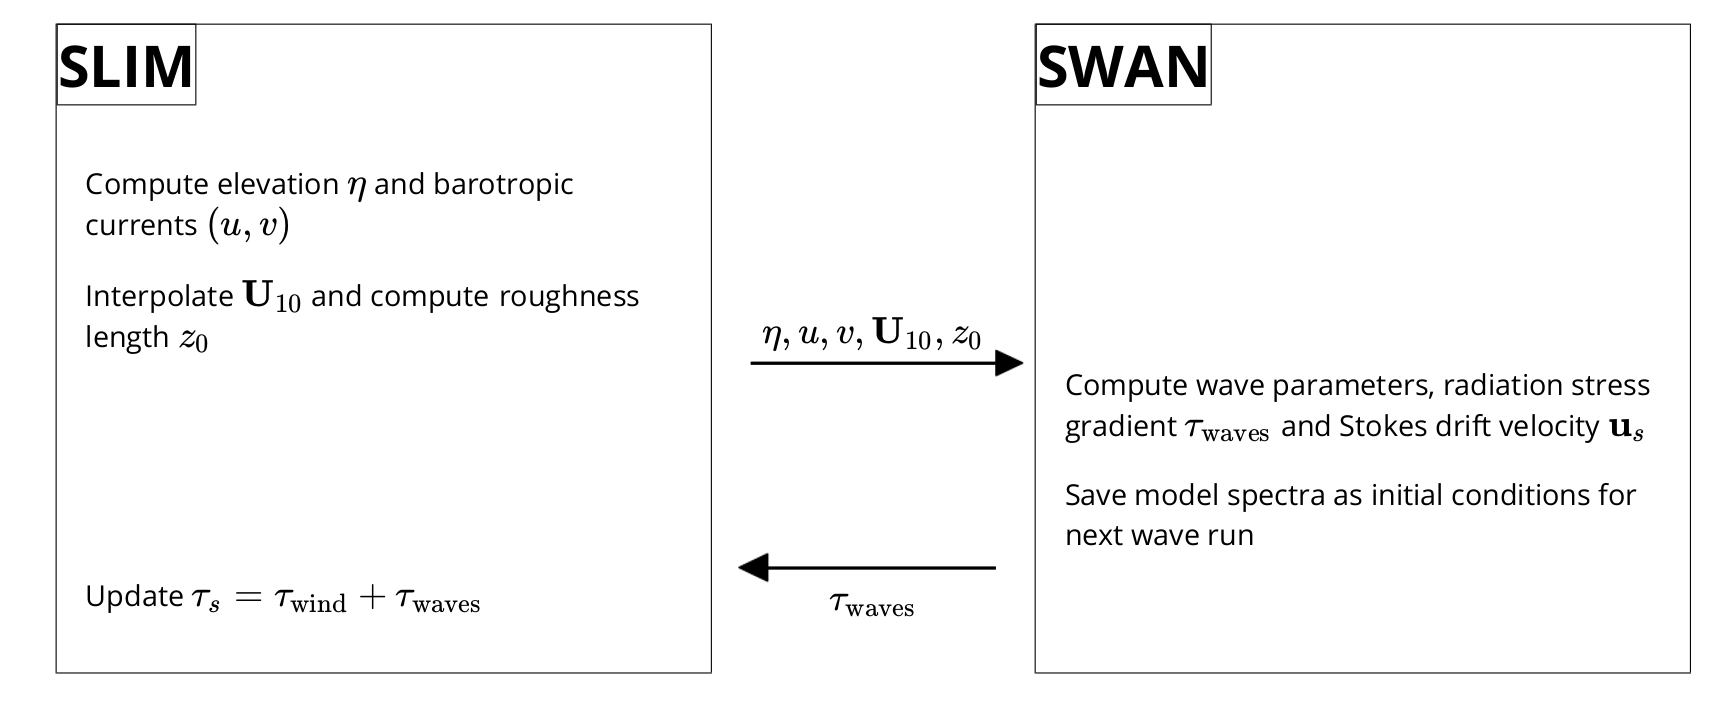
\includegraphics[width=.99\textwidth]{chapters/irma/figures/coupling_v2.png}
    \caption{Schematic illustration of the coupled SLIM+SWAN model.}
    \label{fig:coupling}
\end{figure}

\subsection{Quantifying the effect of wave-current interactions on transport}\label{sec:traj}

To quantify the impact of wave-current interactions on transport processes, we compared the trajectories of passive particles advected by the uncoupled SLIM and coupled SLIM+SWAN currents during the passage of Irma in the Lower Keys. Furthermore, the depth-averaged Stokes drift was computed using the wave spectra of the coupled model SLIM+SWAN run as well as those of an uncoupled SWAN run. Particles were released on the inner and outer shelves at the points highlighted by red and blue dots in Fig. \ref{fig:init} on Sept. 7 at 0000 UTC and then tracked until Sept. 15. These initial particle positions were found using backtracking methods \citep{spivakovskaya2005simulation} to ensure that the release particles would intersect the path of Irma during its passage through the Florida Keys. We first defined two 25 km$^\text{2}$ circular regions on the trajectory of the hurricane (see red and blue circles in Fig. \ref{fig:init}). Particles within these two regions were then tracked backward in time using uncoupled SLIM currents from the exact time of the passage of the hurricane until Sept. 7 at 0000 UTC. Their positions at the end of the backward simulation (see red and blue particle clouds in Fig. \ref{fig:init}) corresponds to the initial condition of the forward transport simulations described below. We then compared the trajectories of particles originating from these regions and advected forward in time by different sets of currents: (i) uncoupled SLIM currents alone; (ii) coupled SLIM+SWAN currents; (iii) SLIM currents with the addition of the depth-averaged Stokes drift computed with the coupled wave-current model (Stokes-C); (iv) SLIM+SWAN currents with Stokes-C; and (v) SLIM currents with the depth-averaged Stokes drift computed with the uncoupled wave model (Stokes-U). The different combinations of Eulerian currents and Stokes drifts used to model the transport of passive drifters in the Lower Keys during the passage of Irma are summarized in Table \ref{tab:summary}. Particle trajectories are compared by computing the distances between the centers of mass of the particle clouds through time.

\begin{figure}
    \centering
    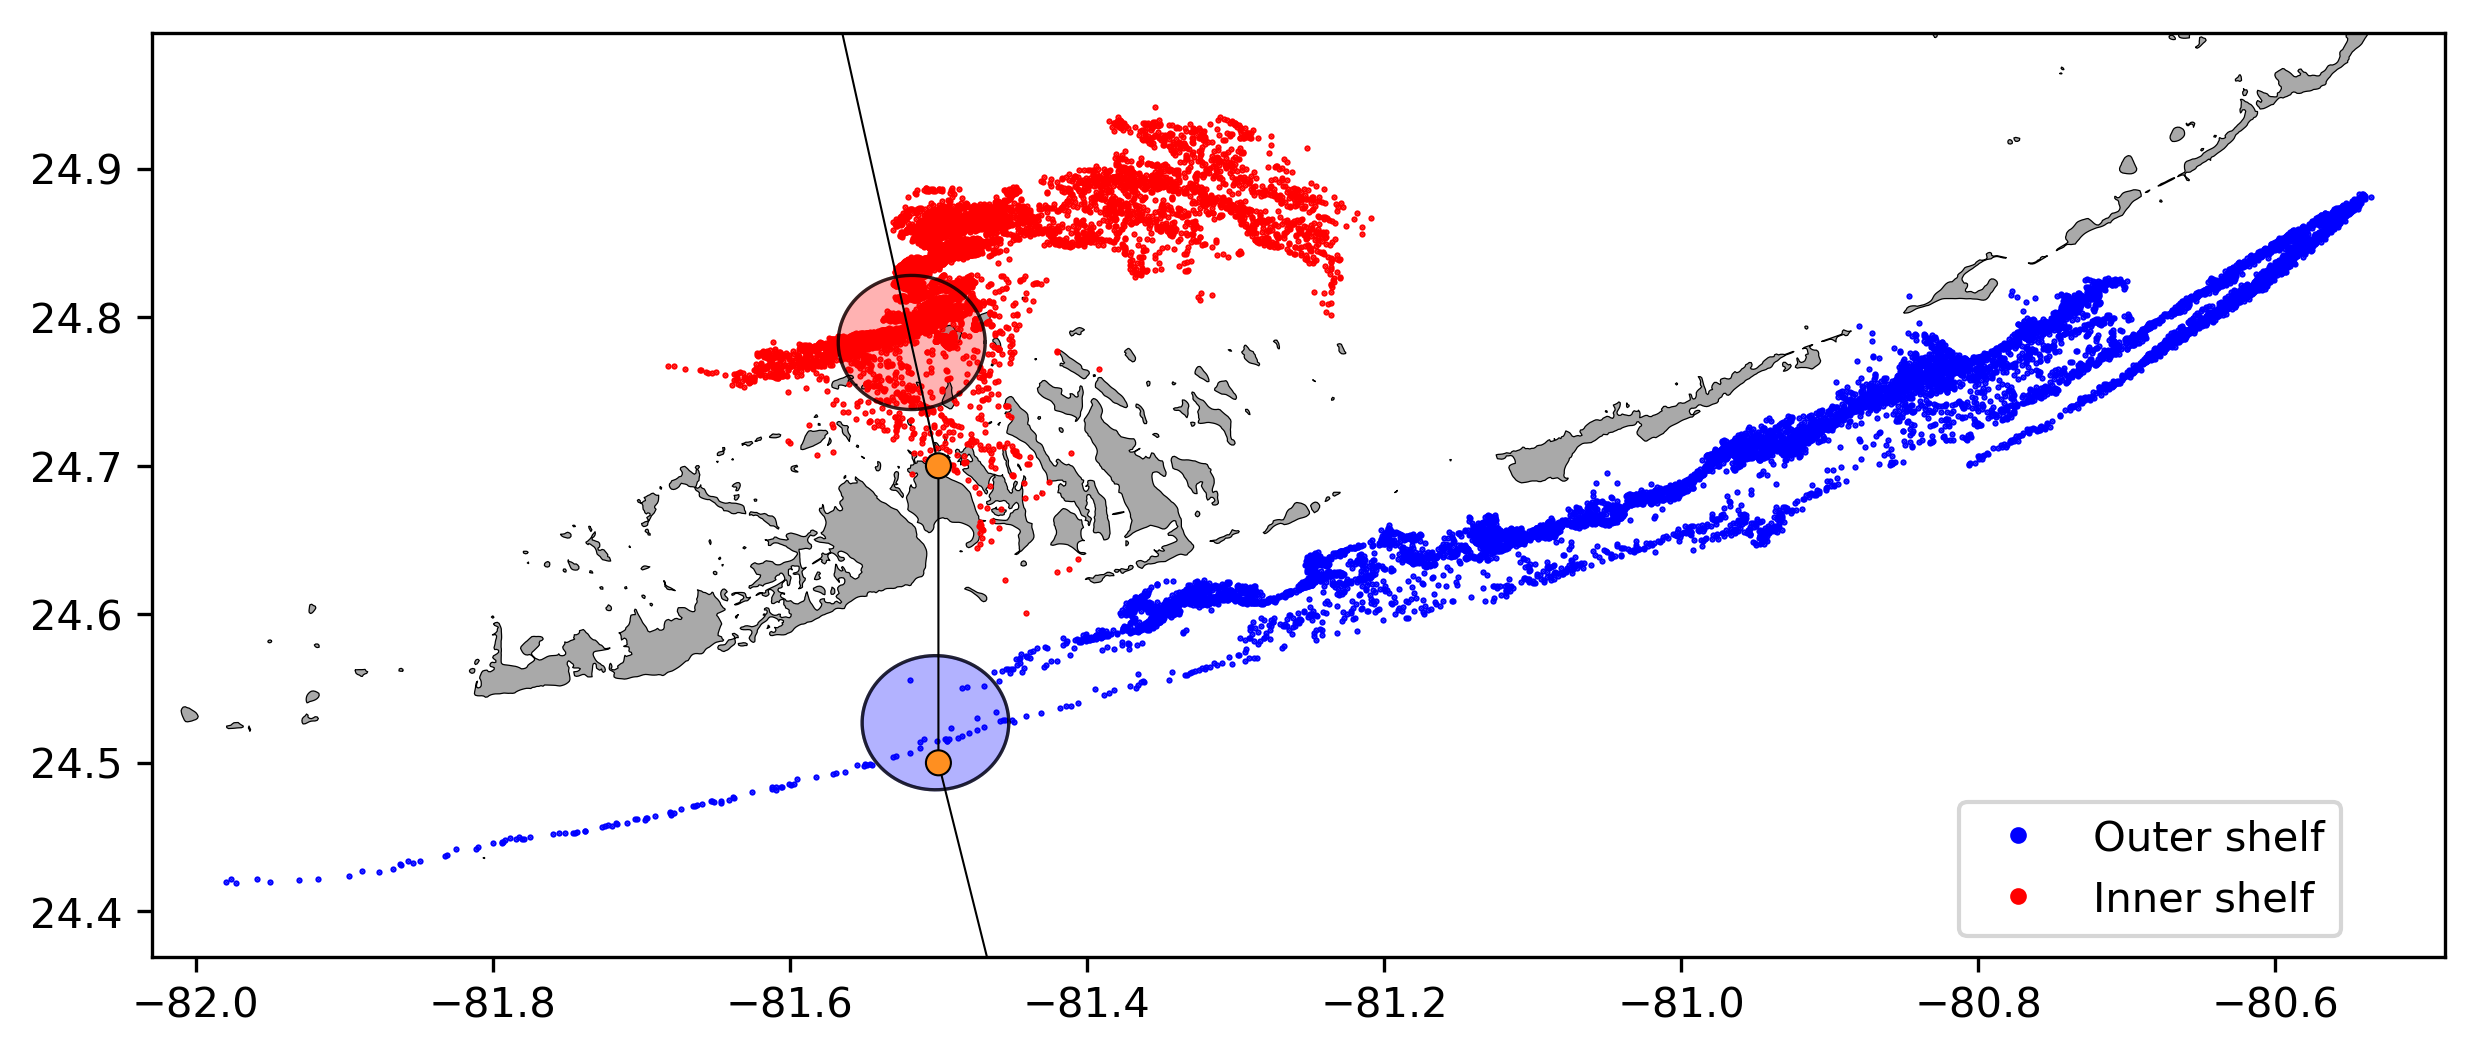
\includegraphics[width=.95\textwidth]{chapters/irma/figures/figure_initial_positions.png}
    \caption{Release regions of the passive particles on the inner and outer shelves on Sept 7 at 0000 UTC (red and blue clouds) obtained by backtracking particles released in the red and blue circular areas during the passage of Irma.}
    \label{fig:init}
\end{figure}

\begin{table}
    \centering
%    \begin{tabular}{|p{4.5cm}|p{8cm}|}
%        \hline
%        \textbf{Experiment name} & \textbf{Model description} \\ \hline
%        SLIM               & Eulerian currents from the uncoupled SLIM simulation \\ \hline
%        SLIM+SWAN          & Eulerian currents impacted by the RS gradient from the coupled SLIM+SWAN simulation \\ \hline
%        SLIM+Stokes-U      & Eulerian currents from the uncoupled SLIM run with the Stokes drift from the uncoupled SWAN simulation \\ \hline
%        SLIM+Stokes-C      & Eulerian currents from the uncoupled SLIM run with the Stokes drift from the coupled SLIM+SWAN simulation \\ \hline
%        SLIM+SWAN+Stokes-C & Eulerian currents impacted by the RS gradient and the Stokes drift from the coupled SLIM+SWAN simulation \\ \hline
%    \end{tabular}
    \begin{tabular}{|p{4.5cm}|p{4cm}|p{4cm}|}
        \hline
        \textbf{Experiment name} & \textbf{Eulerian currents from} &  \textbf{Stokes drift from}\\ \hline
        SLIM               & uncoupled SLIM simulation & None \\ \hline
        SLIM+SWAN          & coupled SLIM+SWAN simulation (impacted by RS gradient) & None \\ \hline
        SLIM+Stokes-U      & uncoupled SLIM simulation & uncoupled SWAN simulation \\ \hline
        SLIM+Stokes-C      & uncoupled SLIM simulation & coupled SLIM+SWAN simulation \\ \hline
        SLIM+SWAN+Stokes-C & coupled SLIM+SWAN simulation (impacted by RS gradient) & coupled SLIM+SWAN simulation \\ \hline
    \end{tabular}
    \caption{Summary of the different combinations of Eulerian currents and Stokes drifts used to model the transport of passive drifters on the passage of Hurricane Irma in the Lower Keys}
    \label{tab:summary}
\end{table}

%%%%%%%%%%%%%%%%%%%
% --- RESULTS --- %
%%%%%%%%%%%%%%%%%%%
\section{Results}

We first validated the reconstructed atmospheric fields of Hurricane Irma as well as the outputs of our coupled wave-current model against field measurements. We then used the validated model outputs to simulate the transport of passive particles in the Lower Keys during the passage of Hurricane Irma. These particles were advected by the sets of currents described in Table \ref{tab:summary} and their trajectories were compared to evaluate the impact of the wave-current interactions and the Stokes drift on the transport processes during the passage of Irma.

\subsection{Model validation}

H*Wind winds and hybrid pressure field agree well with station measurements at Vaca Key station (Fig. \ref{fig:forcings}). The hybrid pressure field shows a better agreement with observations than ERA-5 pressure as it successfully reproduces the storm depression. ERA-5 fields, on the other hand, fail to reproduce the low pressure at the core of the hurricane due to their coarser grid, leading to an overestimation of 8 mbar of the storm depression. Both H*Wind and ERA-5 agree well with observed wind speeds although both data sets tend to slightly overestimate the width and intensity of the wind peak. However, H*Wind profiles better reproduce the timing of the observed peak, as ERA-5 winds tend to anticipate it. H*wind also exhibits a slightly narrower peak in wind speed, which better agrees with observations.

\begin{figure}
    \centering
    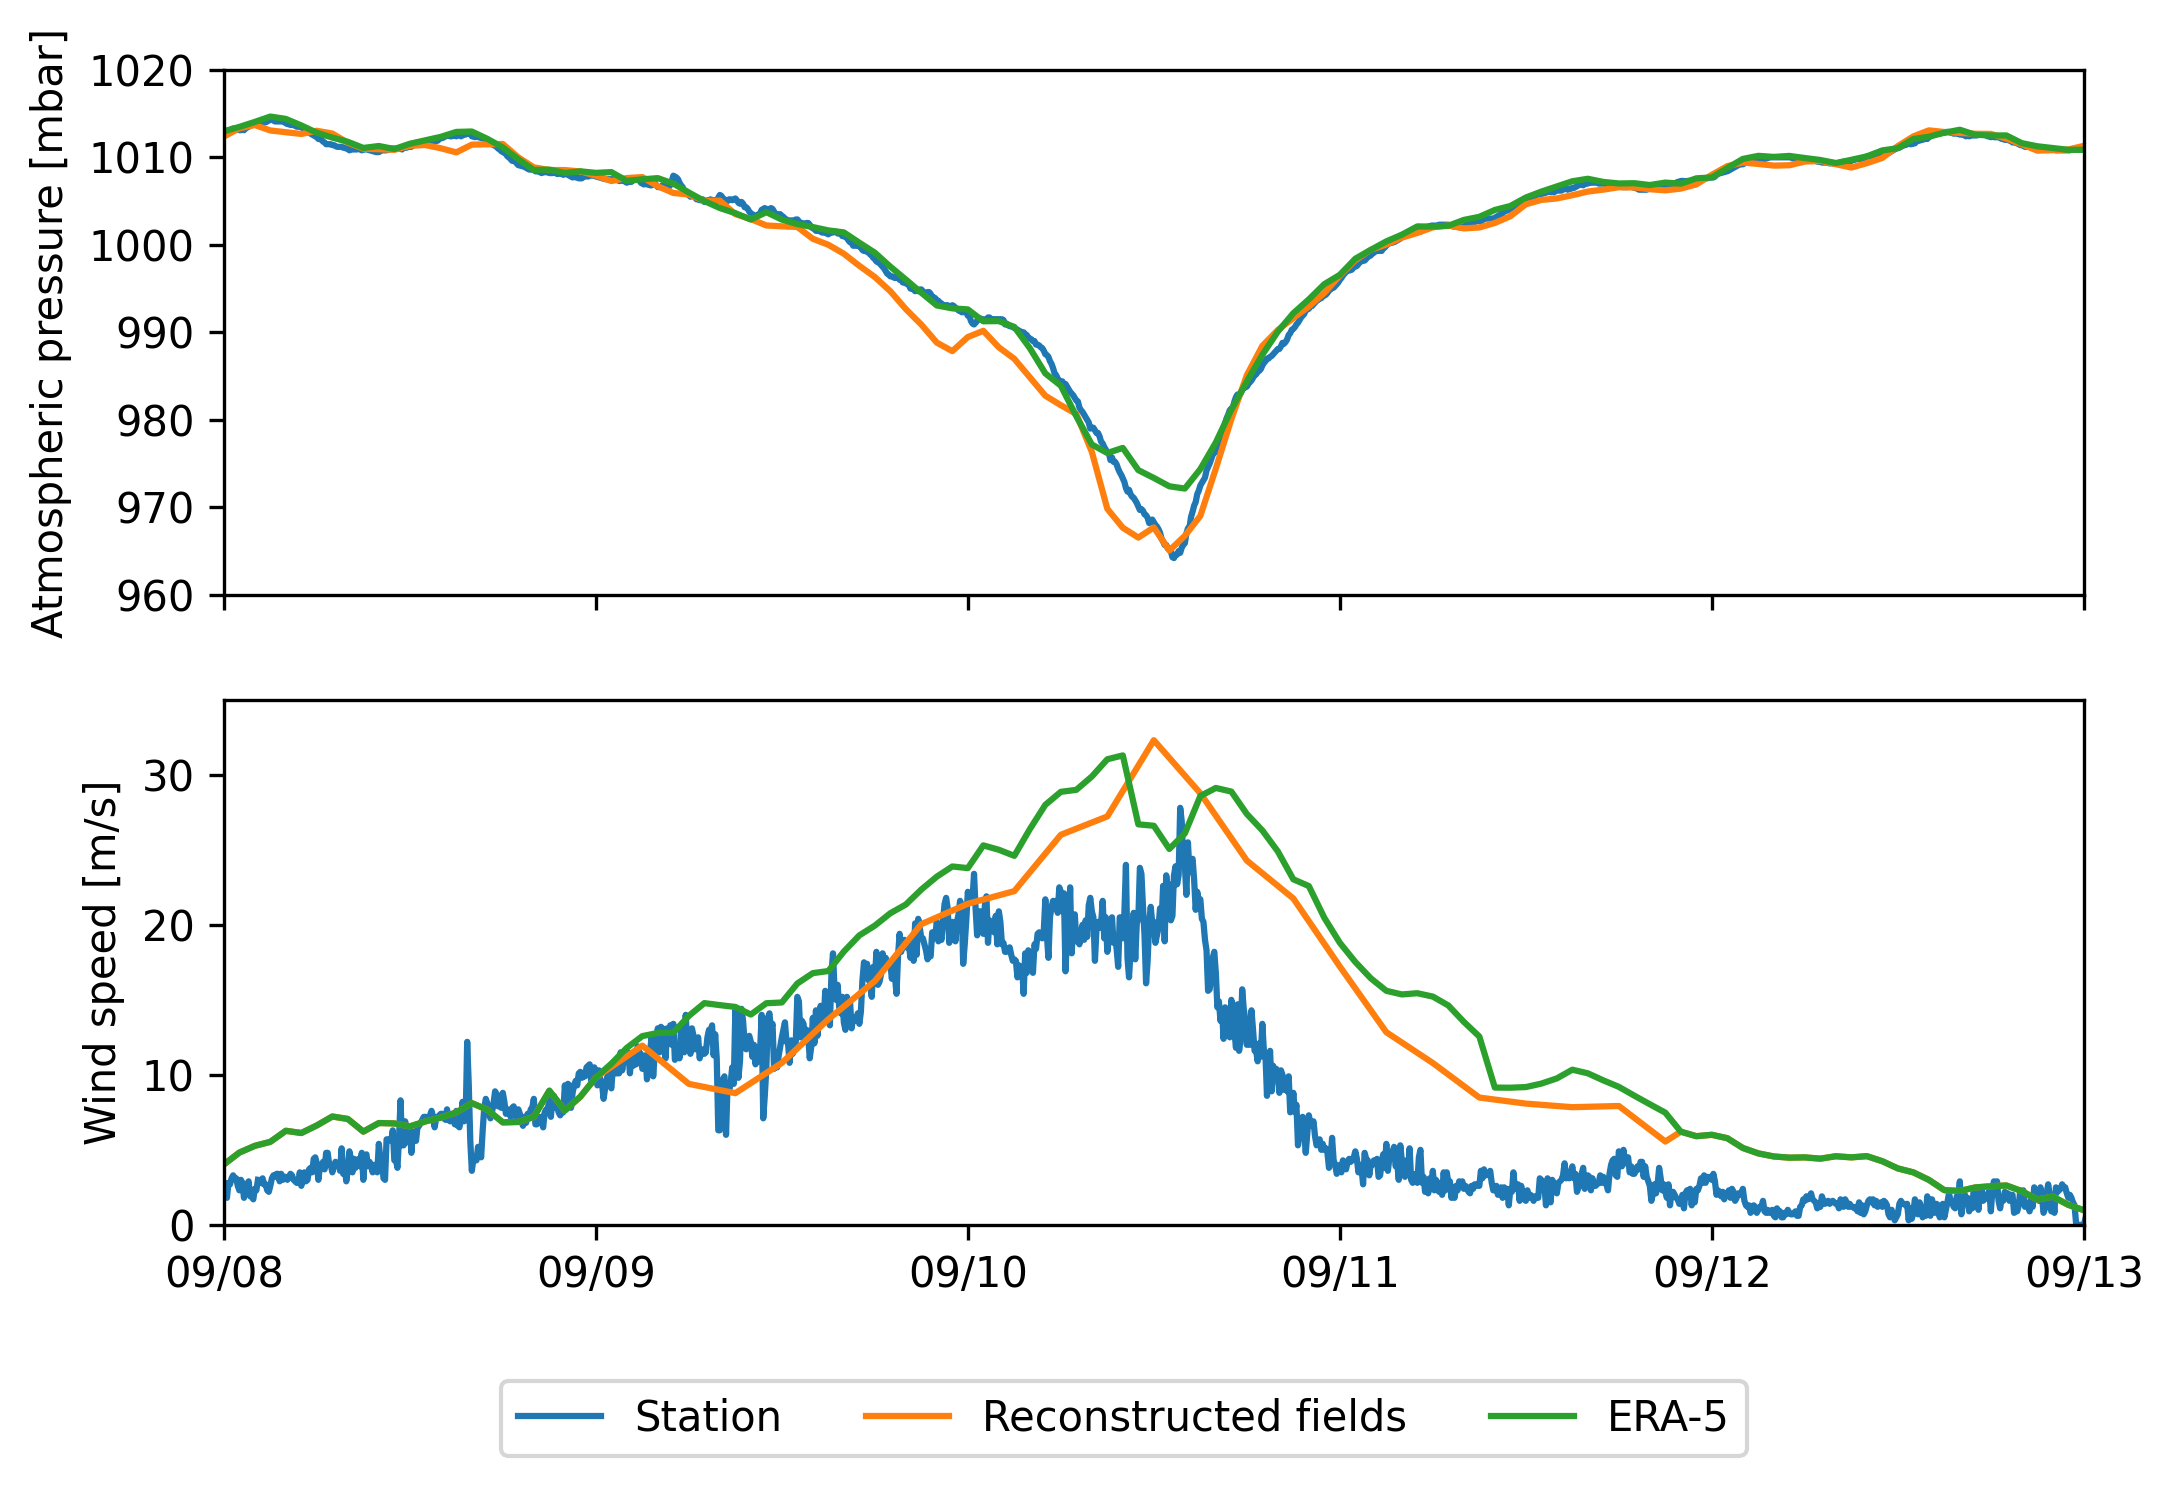
\includegraphics[width=.95\textwidth]{chapters/irma/figures/validation_met_2.png}
    \caption{Comparison of reconstructed atmospheric pressure (top) and wind speed (bottom)} with field measurements and coarser ECMWF ERA-5 profiles at Vaca Key station. The generated hybrid atmospheric forcings better reproduce the observed storm depression while H*wind winds better reproduce the measured peak in wind speed.
    \label{fig:forcings}
\end{figure}

Hydrodynamic outputs of the coupled wave-current model agree well with tide gauge (Fig. \ref{fig:sse}) and ADCP measurements (Fig. \ref{fig:uv}). The coupled model reproduces well the timing of the positive and negative storm surges at all tide gauge locations. The amplitude of the positive surges are especially well captured at Naples and Vaca Key, with errors of 2 and 6 centimeters respectively. However, the model underestimates the positive surges at Virginia Key and Key West by 24\% and 15\% at the peak respectively. The amplitude of the negative surge at Naples is also underestimated by about 16\% at the peak. Nonetheless, on average, the absolute error between the model and observations does not exceed 10 cm (Table \ref{tab:stat}). Modeled 2D currents were validated against depth-averaged ADCP measurements at mooring stations C10, C12 and C13 (Fig. \ref{fig:uv}). As in \cite{liu2020impacts}, we performed the vector correlation analysis of \cite{kundu1976ekman} to compare modeled and observed current velocity vectors. Correlation coefficients ($\rho$) between simulated and observed depth-averaged currents are 0.87, 0.84 and 0.81 at stations C10, C12 and C13, respectively. The average veering angles are below 12$^\circ$, as in \citep{liu2020impacts}. Furthermore, the positive bias in Table \ref{tab:stat} indicates that our model tends to underestimate the southward component of the currents at the different stations. As expected from a depth-averaged model, the best fit with observations is obtained at the shallowest mooring C10, located on the 25 m isobath. 

\begin{figure}
    \centering
    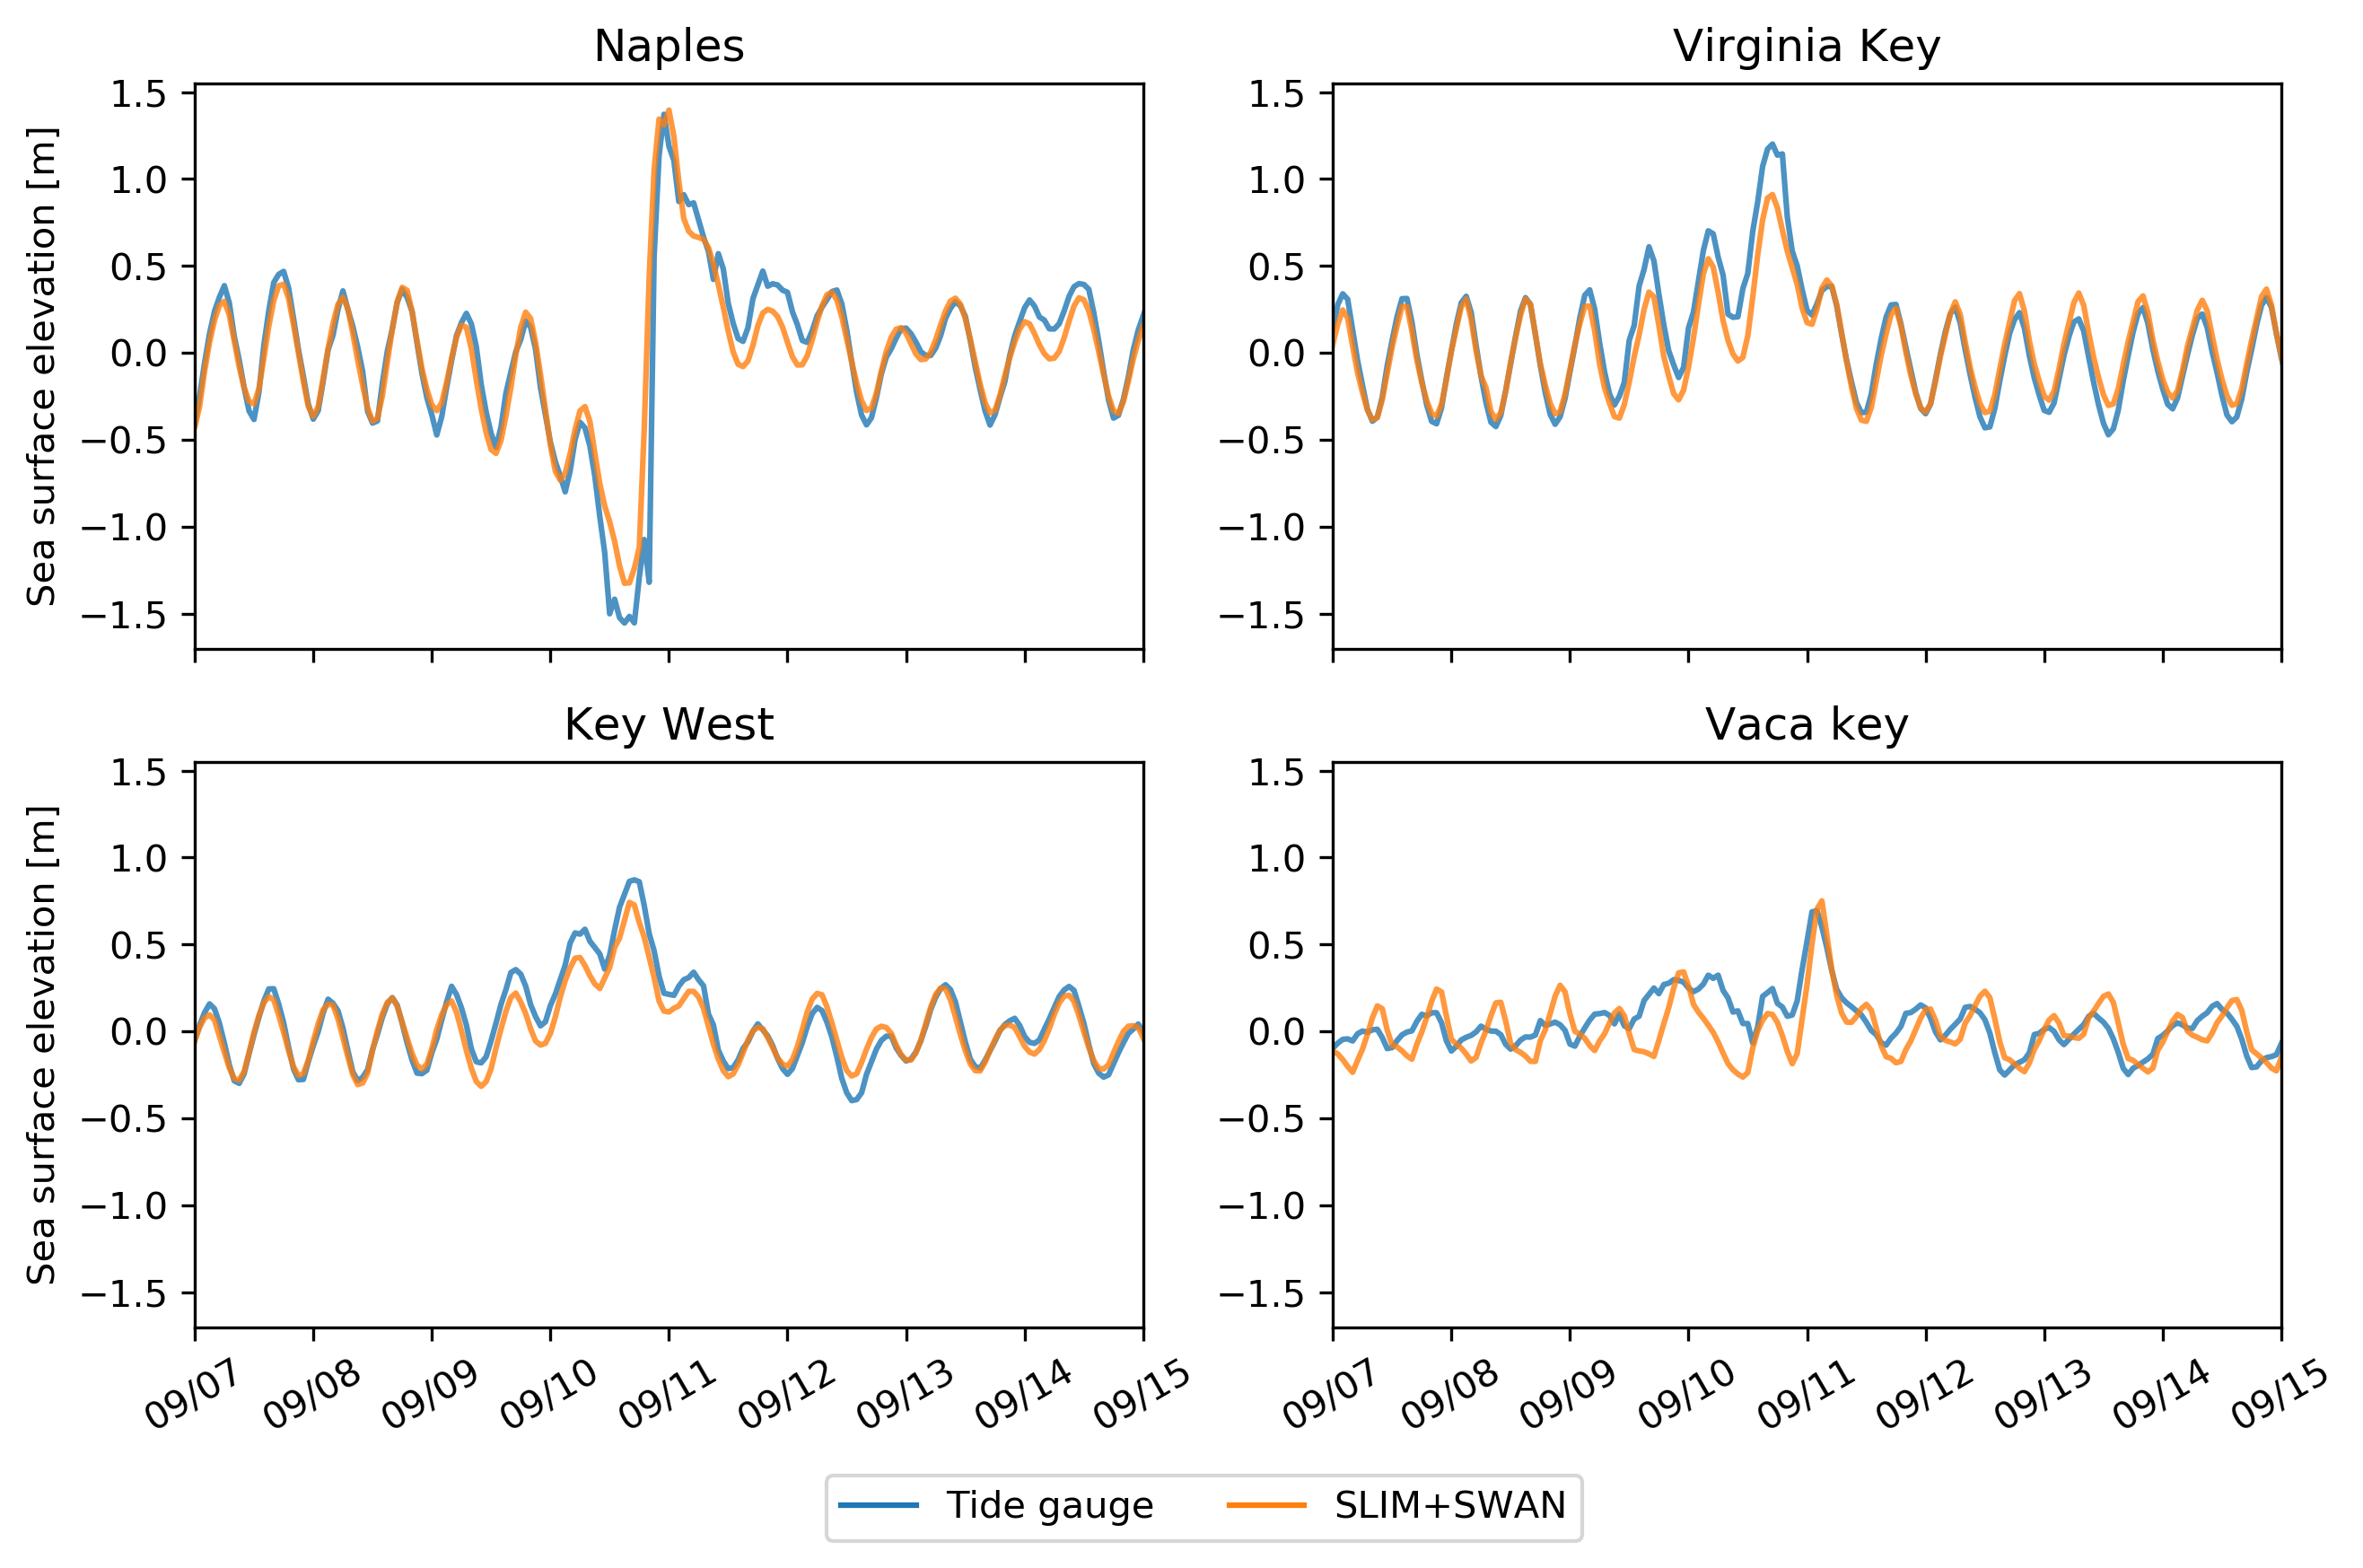
\includegraphics[width=\textwidth]{chapters/irma/figures/validation_eta.png}
    \caption{Comparison of modeled sea surface elevation at the 4 tide gauges shown in Fig. \ref{fig:mesh}B. The timing and amplitude of the storm surges are well reproduced by the model}
    \label{fig:sse}
\end{figure}
\begin{figure}
    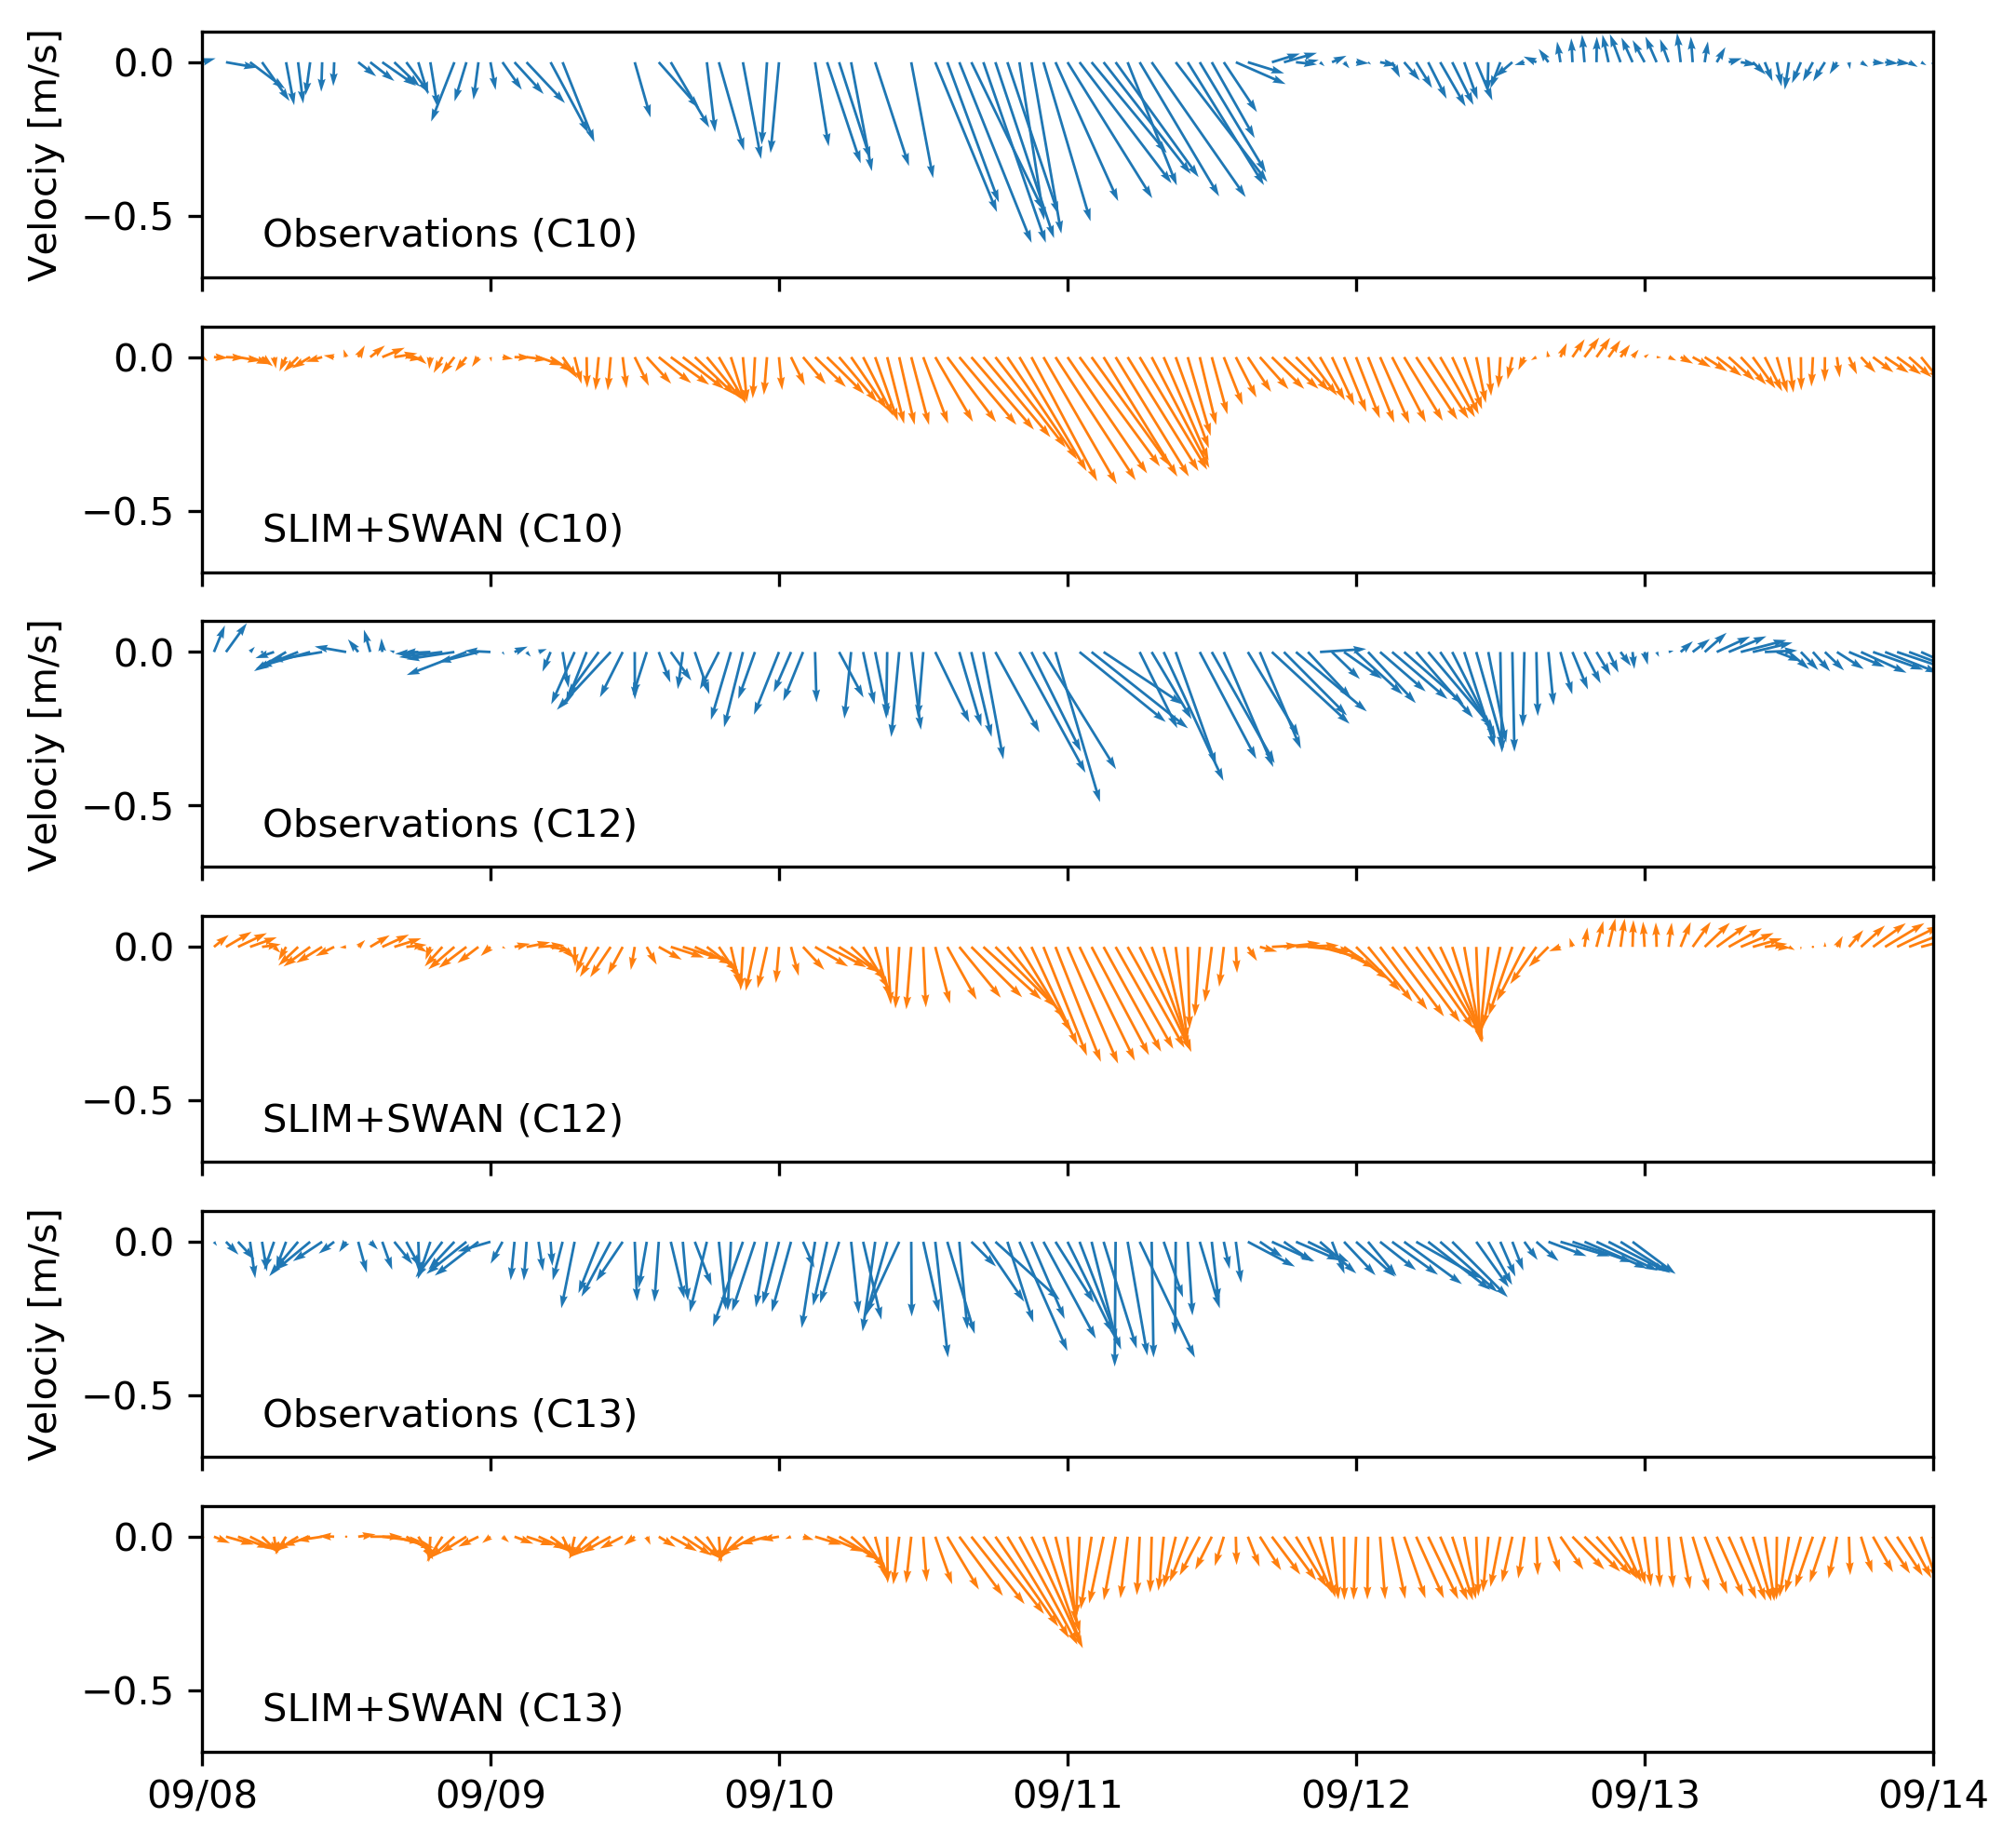
\includegraphics[width=\textwidth]{chapters/irma/figures/figure_currents_all.png}
    \caption{Comparison of modeled current velocity with observed velocity at the moorings (see Fig. \ref{fig:mesh}B for their location). Modeled current velocities agree well with observations, with a correlation coefficient of 0.87, 0.83 and 0.81 at moorings C10, C12 and C13, respectively. The corresponding veering angles are $5.4^\circ$, $0.07^\circ$ and $10.5^\circ$, respectively.}
    \label{fig:uv}
\end{figure}

The simulated significant wave height agrees well with observations at all buoy locations (Fig. \ref{fig:waves}). The timing of the peak in wave height is well captured at all buoys, while the amplitude is better reproduced on the WFS (buoys 42036 and 42097) with errors below 10\%. The error on the peak amplitude on Florida's eastern shelf is of 13\% and 21\% at buoys 4114 and 4113, respectively. On average, observed significant wave height and wave period are better reproduced on the WFS while wave direction is better captured by the model on Florida's eastern shelf (Table \ref{tab:stat}). The fit is especially good at buoy 41113, where the mostly westward-northwestward wave propagation is less perturbed by Irma's wind field.
\begin{figure}
    \centering
    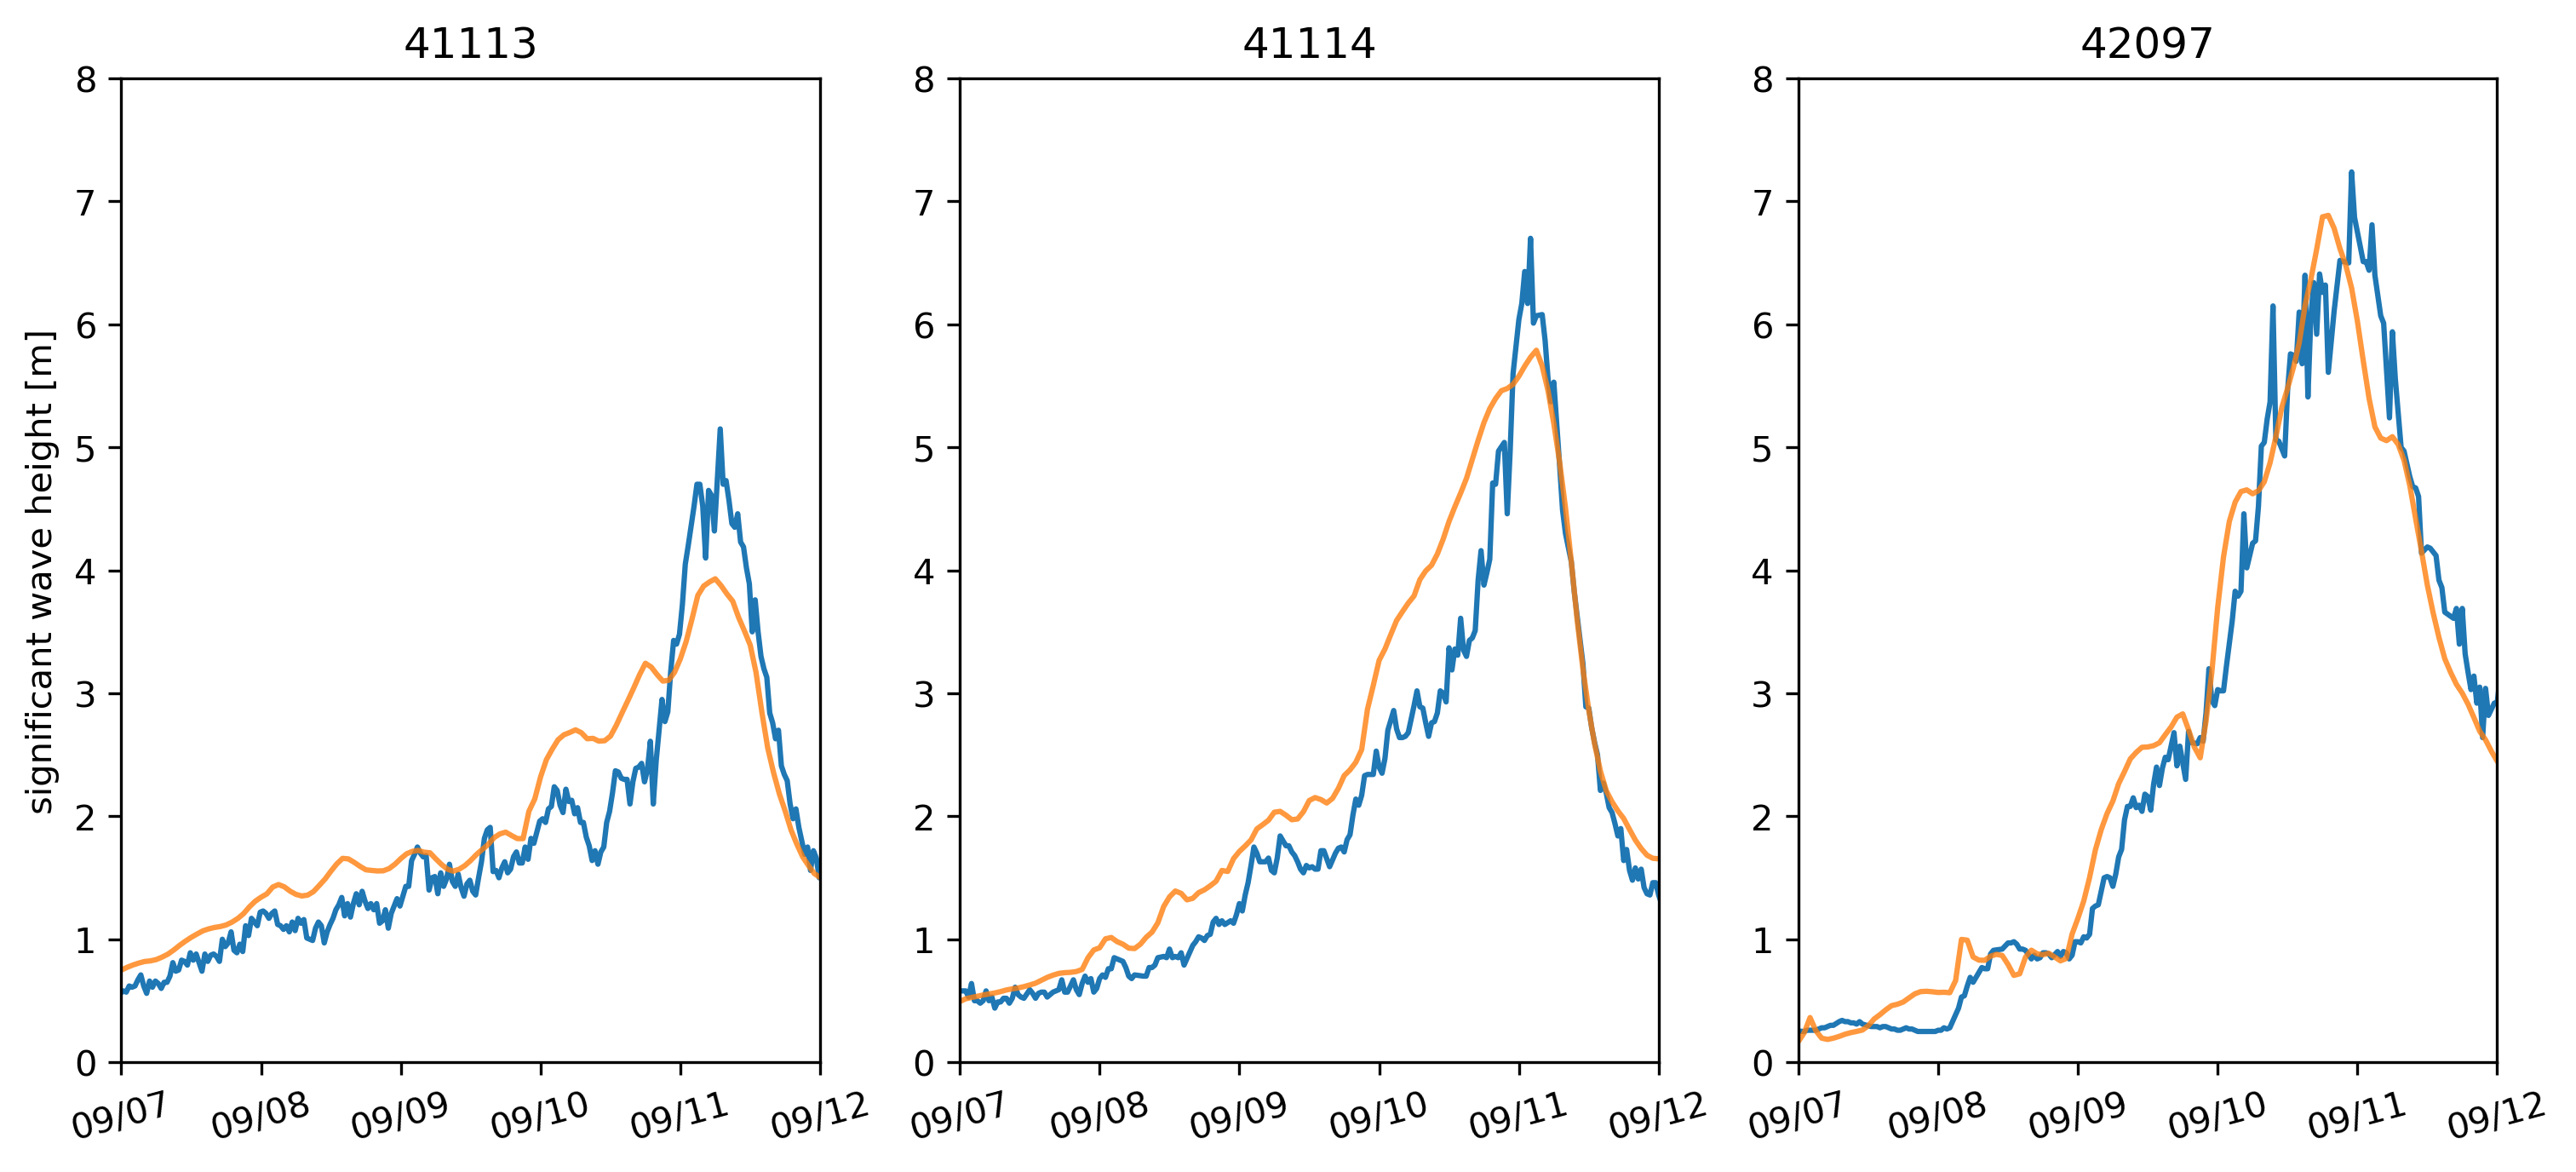
\includegraphics[width=\textwidth]{chapters/irma/figures/hsig_validation.png}
    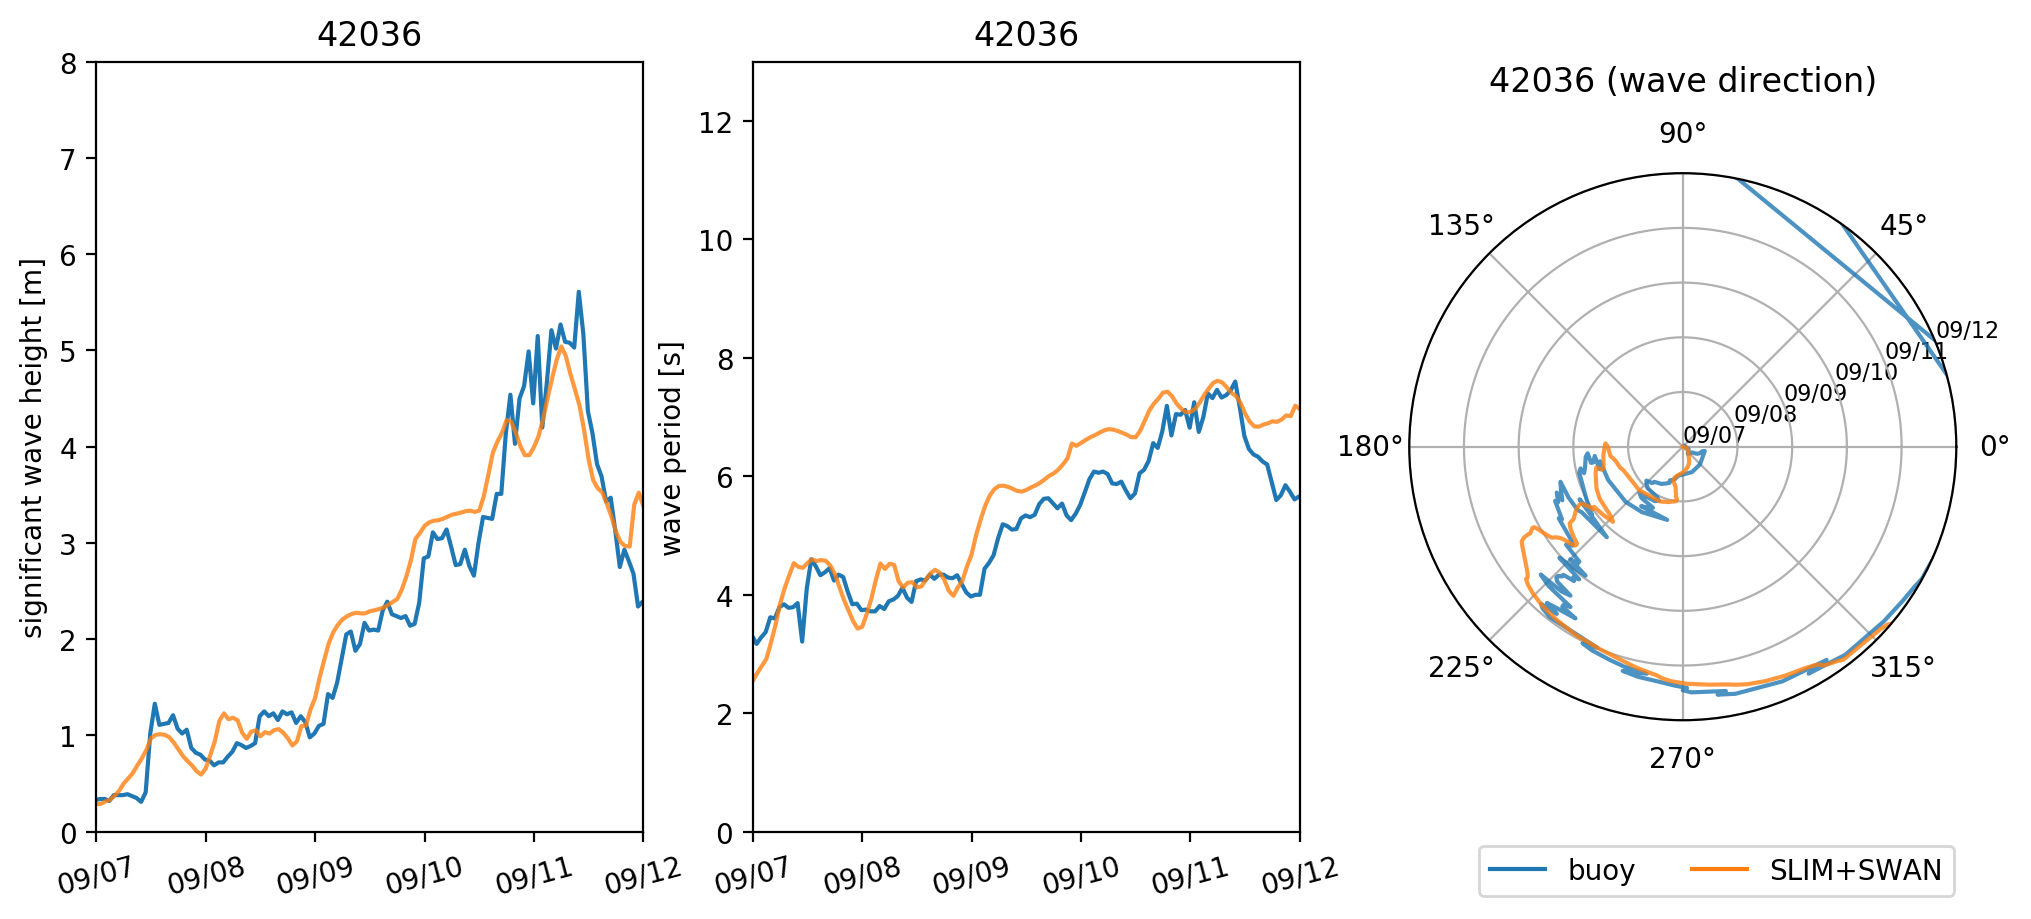
\includegraphics[width=\textwidth]{chapters/irma/figures/wave_validation_42036.png}
    \caption{Comparison of modeled wave parameters with observation at the 4 buoys location (locations shown in Fig. \ref{fig:mesh}B). Overall, the modeled significant wave heights agree well with field measurement (mean error $<25$\%). }
    % As model parameters were calibrated for the Northern Gulf of Mexico, observations are better reproduced at buoys located on the WFS, as illustrated for buoy 42036
    \label{fig:waves}
\end{figure}

\begin{table}
    \centering
    \begin{tabular}{|p{2.8cm}p{3cm}p{1.8cm}p{1.8cm}p{1.8cm}|}
        \hline
        \textbf{Station} & \textbf{Variable} & \textbf{Bias} & \textbf{MAE} & \textbf{RMSE} \\
        \hline
        Vaca Key     & sse (m)              & 0     & 0.112 & 0.142 \\
                     & $U_{10}$ (m/s)       & 1.51  & 1.85  & 2.61 \\
                     & $p_\text{atm}$ (hPa) & -0.21 & 0.59  & 1.03 \\ 
        Key West     & sse (m)              & 0     & 0.066 & 0.085 \\
        Virginia Key & sse (m)              & 0     & 0.087 & 0.120 \\
        Naples       & sse (m)              & 0     & 0.099 & 0.180 \\
        \hline
        C10   & $u$ (m/s)           &  0.002 &  0.045 &  0.056 \\
              & $v$ (m/s)           &  0.039 &  0.102 &  0.121 \\
        C12   & $u$ (m/s)           &  0.002 &  0.059 &  0.074 \\
              & $v$ (m/s)           &  0.047 &  0.073 &  0.094 \\
        C13   & $u$ (m/s)           & -0.009 &  0.065 &  0.077 \\
              & $v$ (m/s)           &  0.039 &  0.086 &  0.102 \\
        \hline
        41113 & $H_s$ (m)           &  0.150 &  0.357 &  0.430 \\
              & $T_m$ (s)           &  1.608 &  1.671 &  1.878 \\
              & $\theta_m$ (degree) & -1.555 &  7.036 &  9.250 \\
        41114 & $H_s$ (m)           &  0.361 &  0.424 &  0.560 \\
              & $T_m$ (s)           &  0.899 &  1.506 &  1.594 \\
              & $\theta_m$ (degree) & -8.236 & 14.616 & 22.560 \\
        42036 & $H_s$ (m)           &  0.082 &  0.312 &  0.398 \\
              & $T_m$ (s)           &  0.430 &  0.528 &  0.645 \\
              & $\theta_m$ (degree) & -2.307 & 17.144 & 22.734 \\
        42097 & $H_s$ (m)           &  0.048 &  0.326 &  0.432 \\
              & $T_m$ (s)           &  0.476 &  0.755 &  0.892 \\
              & $\theta_m$ (degree) &  2.538 & 34.760 & 55.892 \\
        \hline
    \end{tabular}
    \caption{Error statistics on the wave-current model outputs as compared to the measured sea surface elevation (sse), eastward and northward depth-average current velocities ($u$,$v$), significant wave height ($H_s$), zero-crossing mean wave period ($T_m$) and mean wave direction ($\theta_m$). Model bias, mean absolute error (MAE), and root mean squared error (RMSE) are listed by variable (unit) and value.}
    \label{tab:stat}
\end{table}

\subsection{Impact of waves on currents and transport}

We evaluated the impact of the RS gradient on the modeled currents during the passage of Irma in the Lower Keys, between Sept. 7 and 13, 2017. First, we computed the maximum difference between currents modeled by SLIM and SLIM+SWAN during this period (Fig. \ref{fig:diff}A). The largest differences in current speed were observed over the reefs, on the shelf break and around islands. They locally reach 1 m/s, with the coupled SLIM+SWAN model yielding the largest amplitudes. The regions where the differences were the largest correspond to areas that experienced large maximum values of the RS gradient {\boldmath$\tau$}$_\text{wave}$ (Fig. \ref{fig:diff}B). These areas of large RS gradient are located on the shelf break and over coral reefs, where important wave energy dissipation occurred through depth-induced wave breaking and bottom dissipation \citep{longuet1964radiation}. This highlights the important protective role of the barrier formed by the offshore reefs, that require a fine spatial resolution to be accurately represented by the model. RS-induced differences in current speed were amplified by the action of the wind stress {\boldmath$\tau$}$_\text{wind}$ (Fig. \ref{fig:diff}C). Wind speeds were larger in the front right quadrant of the hurricane \citep{zedler2009ocean}, yielding larger differences on the right-hand side of the storm trajectory. This is especially clear in the area between the Florida Keys and the Everglades, where relatively small values of {\boldmath$\tau$}$_\text{wave}$ produce current speed differences larger than 0.5 m/s because of the wind stress.

\begin{figure}
    \centering
    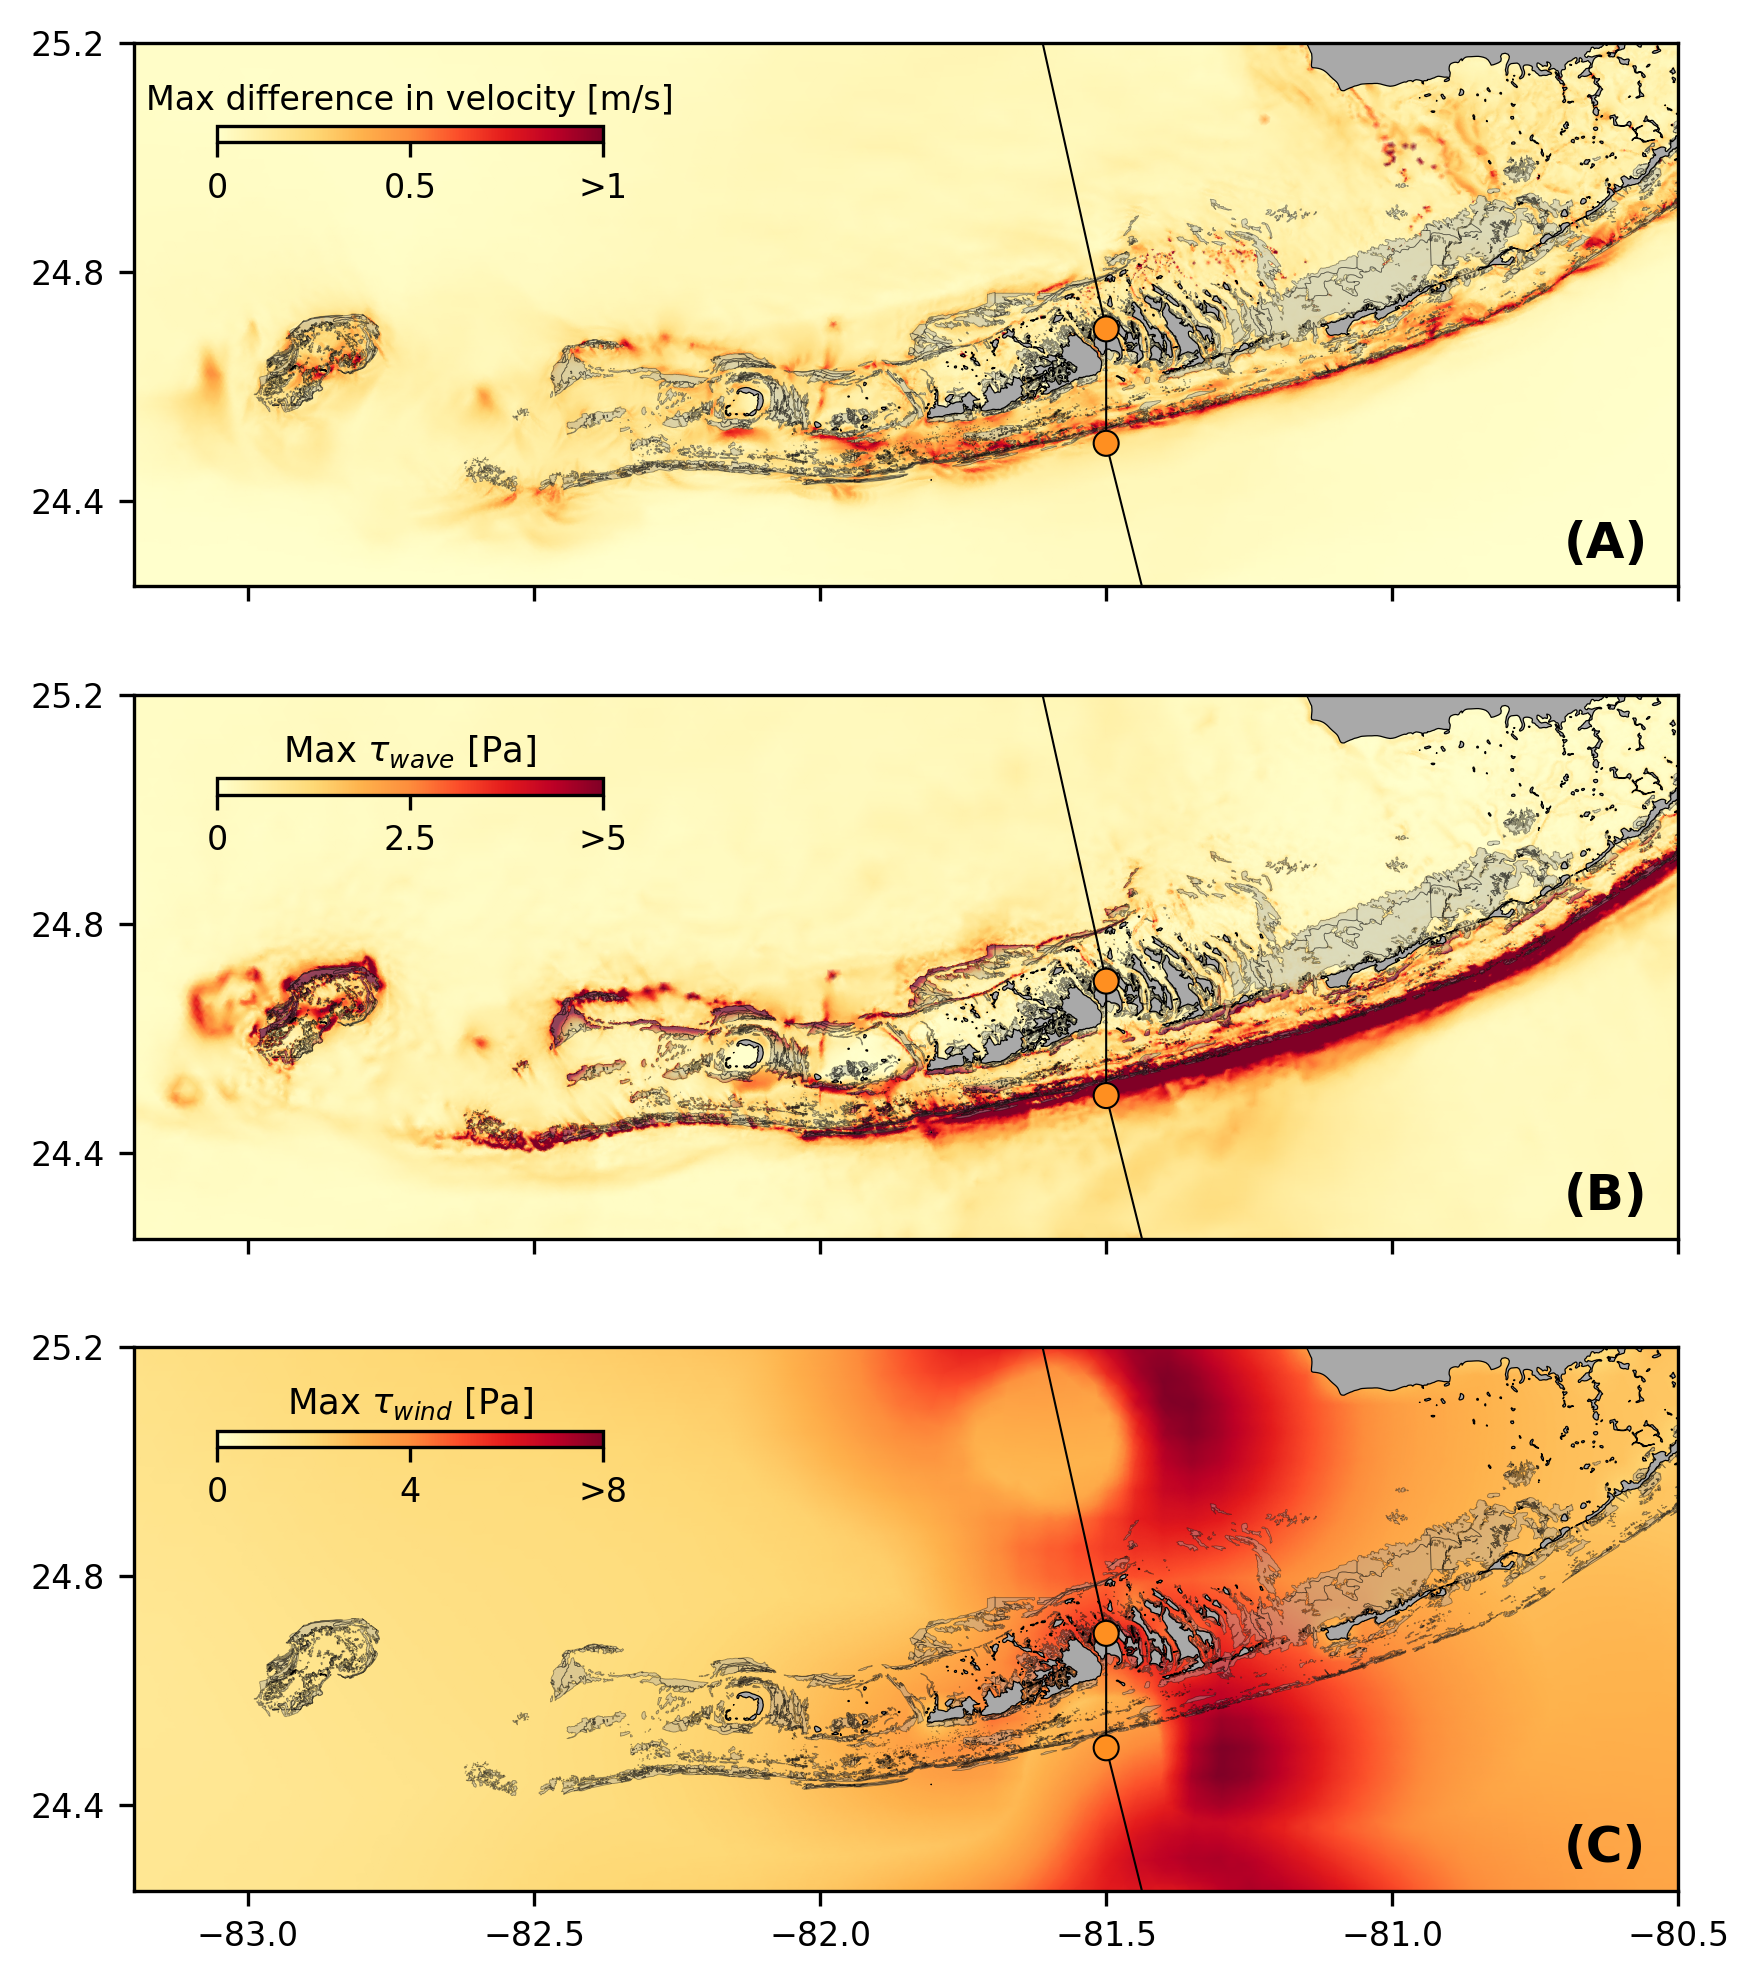
\includegraphics[width=\textwidth]{chapters/irma/figures/max_diff_new.png}
    \caption{(\textbf{A}). Maximum difference between SLIM and SLIM+SWAN currents during the passage of Irma in the Lower Florida Keys; (\textbf{B}) Maximum wave radiation stress gradient {\boldmath$\tau$}$_\text{wave}$ and (\textbf{C}) maximum wind stress {\boldmath$\tau$}$_\text{wind}$ (\textbf{C}) generated by the hurricane. Radiation stress gradient yields currents speed differences reaching 1 m/s, especially over offshore reefs.}
    \label{fig:diff}
\end{figure}

Our results suggest that the RS gradient alone can deflect particle trajectories by up to 1 km on the inner shelf and 5 km on the outer shelf (Fig. \ref{fig:traj}A,B). The RS mainly affects transport processes during the passage of the hurricane, as the distance between particle cloud advected by SLIM and SLIM+SWAN currents remains roughly constant afterwards. The Stokes drift, however, has a longer-lasting effect on the particle trajectories on the outer shelf. When adding a Stokes drift component to the Eulerian currents, the distances between the particle cloud centers keeps increasing during 2 days after the passage of Irma (Fig. \ref{fig:traj}B). Under the effect of the Stokes drift, particles from the outer shelf can be moved inshore on the passage of the hurricane. This motion is less pronounced for particles that are advected by Eulerian currents only. The particle cloud thus moves quickly northeastward under the action of the FC. After 2 days, the particles advected inshore under the action of the Stokes drift are in turn entrained by the FC and the distance between the clouds of particles starts decreasing. The impact of the Stokes drift on particle motion appears to be five times larger than the one of the RS on the inner shelf (Fig. \ref{fig:traj}A). However, both processes yield a similar impact on the particle trajectories at the moment of the passage of Hurricane Irma on the outer shelf (Fig. \ref{fig:traj}B).

Taking wave-currents interactions into account appears to significantly impact the modeled Stokes drift (Fig. \ref{fig:traj}C,D). Our results suggest that neglecting the wave-current coupling when computing the Stokes drift in storm conditions can yield deflections of the particle trajectories by up to 5 km on both the inner and outer shelves. On the outer shelf, differences in particle trajectories mostly appear during the two days following the passage of the hurricane. This is explained by the stronger shoreward component of the coupled SLIM+SWAN Stokes drift compared to the uncoupled one. On the inner shelf, however, differences in particle trajectories of up to 5 km occur at the moment of the passage of Hurricane Irma. The distance between the particle clouds then stabilizes directly after the passage of the hurricane.

% Milan: Table in complement of graph for comparison of trajectories ?

\begin{figure}
    \centering
    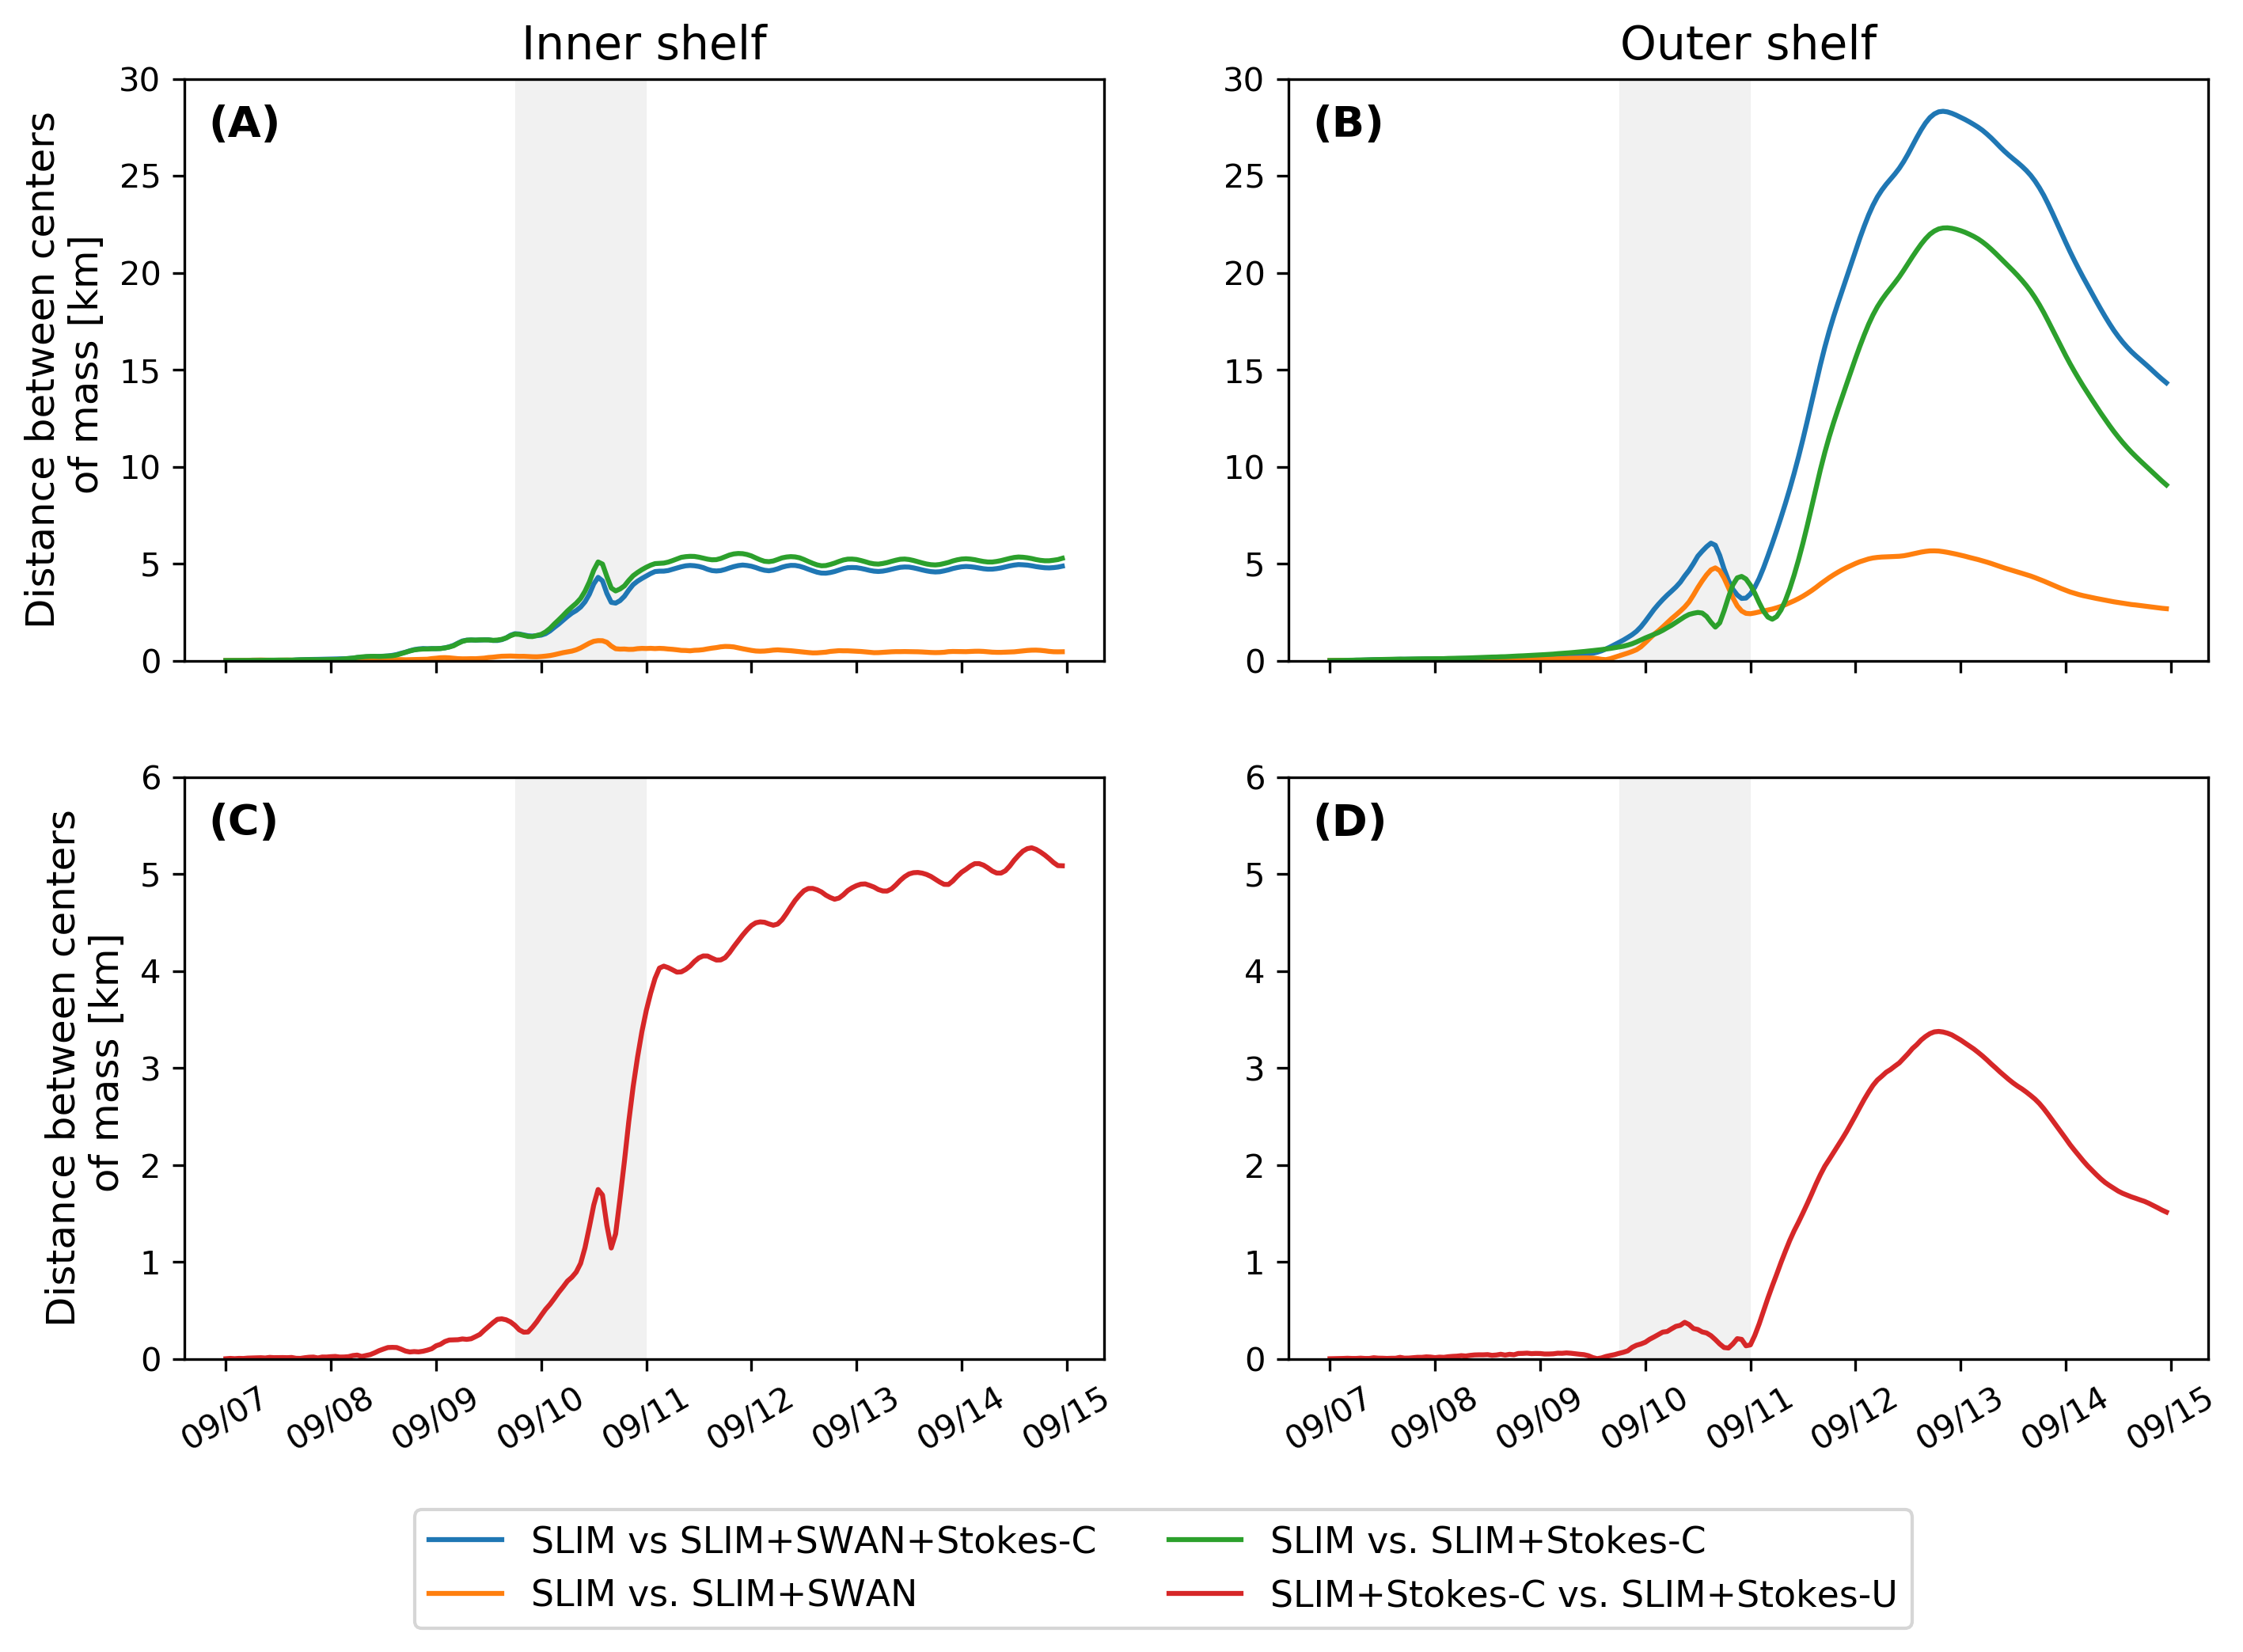
\includegraphics[width=.99\textwidth]{chapters/irma/figures/trajectory_comparisons.png}
    \caption{Difference between the centers of mass of the particle clouds released from the regions highlighted in Fig. \ref{fig:init} and advected by the different combinations of Eulerian currents and Stokes drifts described in Table \ref{tab:summary}}.
    \label{fig:traj}
\end{figure}

% \begin{figure}
%     \centering
%     \includegraphics[width=.98\textwidth]{fig/dispersion.png}
%     \caption{Dispersion of particles with different velocity fields $\rightarrow$ not sure to know what to say about that...}   
%     \label{fig:dispersion}
% \end{figure}

% === DISCUSSION === %
\section{Discussion}
% SUMMARY
The coupled SLIM+SWAN model correctly reproduced the hydrodynamics and wave dynamics during Hurricane Irma. Such good agreement with field measurements could only be achieved using accurate forcings and adequate wave parameterizations. By comparing coupled and uncoupled model runs, we showed that neglecting wave radiation stress gradient can induce differences of up to 1 m/s in modeled current velocities. The radiation stress gradient during the hurricane was especially large over the shelf break, where waves are strongly dissipated by the offshore coral reef barrier. The radiation stress gradient alone can deflect drifting particles by up to 5 km during the passage of the hurricane. The impact of the Stokes drift dominates the effects of the radiation stress gradient on transport processes, except during the passage of the hurricane, when both contributions are similar on the outer shelf. The Stokes drift induces a shoreward transport during the passage of the hurricane that moves particles towards  the inner shelf, and hence away from the FC. Finally, neglecting wave-current interactions when computing Stokes drift leads to variations of up to 5 km in modeled trajectories on the passage of the hurricane.

The coupled wave-current model correctly reproduced the timing of the observed storm surges and captured the elevation peaks with a 15\% accuracy at every tide gauge except Virginia Key. Such accuracy is key to predict the damages caused by the hurricane, as they were mostly due to the storm surge and  high waves \citep{xian2018brief}. Furthermore, by using a high-resolution model, we can explicitly reproduce the circulation between all the reefs and islands of the Florida Keys. The fine-scale details of the storm surge, and hence the associated risk, are thus accurately represented. In addition to accurately capturing positive surges, the model also reproduced the observed negative surge in Naples. This result is of interest from a biological point of view as negative surges, although less studied, affect water exchanges between the estuaries and the coastal ocean and disturb the benthic ecosystems \citep{liu2020impacts}. Such rapid decrease in water level followed by a positive surge cause massive freshwater inflows, causing a significant decrease in water salinity \citep{wachnicka2019hurricane}. Surface waters are also significantly impacted by storms and hurricanes through induced cooling, upwelling and mixing \citep{varlas2020investigating}, but these processes were not accounted for in our model.

Strong currents such as the Gulf Stream affect waves through refraction over gradients in current velocity, shoaling and breaking of opposing waves or lengthening of following waves \citep{hegermiller2019wave}. Under hurricane conditions, these interactions can cause numerical instabilities in the wave model if the parameterizations are not appropriate and the model resolution not sufficient. \cite{hegermiller2019wave}, for instance, used a 5-km model grid and 48 directional bins to capture spatial gradients in wave height induced by wave-currents interactions in the Gulf Stream during Hurricane Matthew (2016). We followed these guidelines when defining the coarsest mesh resolution as the wave model spectral discretization. Boundary conditions and directional spreading of the incident waves also play a significant role when modeling wave-current interactions at meso- and submesoscales \citep{villas2020wave}, which motivated our choice of imposing full spectra on the boundary of the wave model instead of bulk parameters.

Tropical cyclones interact with the Gulf Stream and the FC through cooling and mixing of the upper ocean. These interactions can momentarily disrupt these currents and cause a significant reduction of their transport \citep{oey2007hurricane,ezer2017observations,ezer2020long}. As a 2D barotropic model, SLIM does not explicitly capture the vertical structure of the FC and Gulf Stream. Furthermore, a coupling with an atmospheric model would be required to represent heat fluxes between the upper ocean and the hurricane. However, we argue that a 2D model is sufficient for the scope of this study, that focuses on nearshore processes on the shelf and the shelf slope. Furthermore, by coupling the model with HYCOM, SLIM is able to represent indirectly the baroclinic features such as the meandering of the FC and eddie formation \citep{frys2020fine}. Furthermore, using a 2D model allows us to capture the impact of wave-current interactions on transport processes at the reef scale in the topologically complex coastal system of the FRT. Such a fine resolution is key to estimate the amount of wave energy dissipated over offshore reefs and accurately capture the generated RS gradient.

%Finally, SWAN default parameterizations for wind energy input and whitecapping caused numerical instabilities by overestimating wave growth and steepness on the boundary of the Gulf Stream on the passage of Irma. This overestimation was solved by using the parameterization of \cite{siadatmousavi2011evaluation}. The parameters used in this study were calibrated on the Northern Gulf of Mexico conditions, which might explain that our model better reproduces wave parameters at buoys located on the WFS. However, these calibrated parameters might underestimate wind-induced wave growth on Florida's eastern shelf. Consequently, incident wave do not receive enough energy to grow after breaking on the bank boundary, leading to an underestimation of the significant wave height at buoys located on Florida's eastern shelf. A more extensive calibration study might therefore be necessary to further improve the agreement with field measurements on both sides of Florida. Nonetheless, as this study focuses on the wave produced by Irma, which made landfall on the West coast of Florida, the use of parameterizations calibrated for the Gulf of Mexico seems reasonable.

The RS gradient significantly impacts currents during the passage of the hurricane. It can induce differences of up to 1 m/s in the current speed on the shelf break. In this region, waves are strongly dissipated due to action of depth-induced breaking and bottom dissipation on coral reefs. This link between wave breaking, RS gradient and wave-induced nearshore currents is consistent with previous studies on wave-current dynamics during storms \citep{mao2017dynamics,mao2018wave,mao2020particle}. Furthermore, our results highlight the protective role of coral reefs against strong incoming waves \citep{lowe2005spectral}, which requires a sufficiently fine spatial resolution to be explicitly represented in the model. As wave energy mostly dissipates on the shelf break, the impact of the RS gradient on transport processes is 5 times larger on the outer shelf. In the sheltered area of the inner shelf, wave impact on transport processes is dominated by the Stokes drift. Trajectory deflection under the influence of wave-induced motions mostly occurs at the moment of the passage of the hurricane on the inner shelf. After that moment, the distance between the clouds of particles remained roughly constant through time. On the outer shelf, RS and Stokes drift have a similar impact on transport processes at the moment of the passage of the cyclone and deflect particle trajectories by up to 5 km. However, by inducing shoreward transport, the Stokes drift delayed the advection of particles by the FC, therefore causing differences in trajectories of up to 20 km during the days following the passage of the hurricane. The dominance of the Stokes drift on particle transport in storm conditions was also observed in Lake Michigan by \cite{mao2020particle}. Finally, neglecting wave-current coupling in Stokes drift computation leads to differences in modeled trajectories of the order of 5 km on both the inner and the outer shelves. This fact, coupled with the impact of RS-induced currents strongly advocates for the use of coupled wave-current models when studying transport processes in storm conditions.

%Due to the dissipation of incoming waves on the reefs, wave impact during Irma is different on the inner and outer shelves. It is less important on the inner shelf because of the sheltering of the inner shelf due to reefs and islands as well as wave breaking on the shelf break. The inner shelf hence experiences weaker waves and currents, inducing weaker and more localized transport. Furthermore, the impact of winds on waves is reduced in shallower areas under the action of depth-induced breaking. This might explain why differences between particle trajectories stabilize on the inner shelf just after the passage of Hurricane Irma. However, the Florida Keys still experienced strong winds after the passage of the core of the hurricane, which generated high waves in the deeper areas. This might explain why the differences between the modeled trajectories kept increasing on the outer shelf under the action of strong Stokes drift up to two days after the passage of the hurricane.

\section{Conclusion}

We developed a coupled wave-current model to study the impact of waves on transport processes during Hurricane Irma. In order to accurately represent the wind and pressure profiles of the hurricane, we built hybrid fields by combining coarser ERA-5 data with high-resolution H*Wind data for the wind speed and idealized Holland profiles for the pressure. Comparing these hybrid profiles with field observations showed that they were better at reproducing the observed central depression of the hurricane as well as the peak in wind speed than ERA-5 data. Using these hybrid fields as forcings, our coupled model accurately reproduced the storm surge at tide gauge locations and produced currents and wave parameters in good agreement with field observations. The modeled currents and Stokes drift were then used to evaluate the impact of wave-current coupling on the modeled trajectories of passive drifters on the passage of the hurricane through the Florida Keys. Our results show that waves had a significant impact on heavy-wind transport processes and caused deflections of the drifters trajectories by more than 20 km on the outer shelf.

Despite its good agreement with observations, our model could be further refined by improving the representation of wind-wave interactions. In particular, we did not consider the momentum loss due to the action of surface waves, which can lead to overestimations of the momentum flux from the atmosphere to the ocean under hurricane conditions. Our model could therefore be further improved by using a wave-dissipative stress instead of the full wind stress as the momentum flux from the atmosphere to the ocean. As a 2D barotropic model, SLIM does not explicitly represent heat fluxes between the ocean and the atmosphere and the vertical structure of the ocean. However, our study focused on relatively shallow and vertically homogeneous coastal waters using a reef-scale resolution throughout the whole FRT. Such fine resolution allows to explicitly represent wave dissipation over coral reefs and is only achievable using a 2D model due to computational resource limitations.

Wave coupling needs to be taken into account during heavy-wind events but not necessarily in milder conditions. While the RS gradient plays an important role and can lead to differences of up to 5 km, the Stokes drift is about 4 times more intense and is thus the most important wave-induced transport process. Nonetheless, neglecting wave-current coupling through RS when modeling Stokes drift leads to differences of up to 5 km in predicted drifter trajectories. Such discrepancies reveal the strong influence of wave-current interactions on transport under storm conditions. This study brings new insight on the impact of waves on the transport processes nearshore during a tropical cyclone. Due to its fine spatial resolution, our coupled wave-current model can be used to accurately represent the dispersal of pollutants, sediments or larvae in topologically complex coastal areas in heavy-wind conditions.  
